%%%%%%%%%%%%%%%%%%%%%%%%%%%%%%%%%%%%%%%%%%%%%%%%%%%%%%%%%%%%%%%%%%%%%%%%%%%%%%%%
%% Plantilla de memoria en LaTeX para la ETSIT - Universidad Rey Juan Carlos
%%
%% Por Gregorio Robles <grex arroba gsyc.urjc.es>
%%     Grupo de Sistemas y Comunicaciones
%%     Escuela Técnica Superior de Ingenieros de Telecomunicación
%%     Universidad Rey Juan Carlos
%% (muchas ideas tomadas de Internet, colegas del GSyC, antiguos alumnos...
%%  etc. Muchas gracias a todos)
%%
%% La última versión de esta plantilla está siempre disponible en:
%%     https://github.com/gregoriorobles/plantilla-memoria
%%
%% Para obtener PDF, ejecuta en la shell:
%%   make
%% (las imágenes deben ir en PNG o JPG)

%%%%%%%%%%%%%%%%%%%%%%%%%%%%%%%%%%%%%%%%%%%%%%%%%%%%%%%%%%%%%%%%%%%%%%%%%%%%%%%%

\documentclass[a4paper, 12pt]{book}
%\usepackage[T1]{fontenc}

\usepackage[a4paper, left=2.5cm, right=2.5cm, top=3cm, bottom=3cm]{geometry}
\usepackage{times}
\usepackage[utf8]{inputenc}
\usepackage[spanish]{babel} % Comenta esta línea si tu memoria es en inglés
\usepackage{url}
%\usepackage[dvipdfm]{graphicx}
\usepackage{graphicx}
\usepackage{float}  %% H para posicionar figuras
\usepackage[nottoc, notlot, notlof, notindex]{tocbibind} %% Opciones de índice
\usepackage{latexsym}  %% Logo LaTeX

\usepackage{listings}
\usepackage{color}

% Para mostrar código
\definecolor{dkgreen}{rgb}{0,0.6,0}
\definecolor{gray}{rgb}{0.5,0.5,0.5}
\definecolor{mauve}{rgb}{0.58,0,0.82}

\lstset{frame=tb,
  language=XML,
  aboveskip=3mm,
  belowskip=3mm,
  showstringspaces=false,
  columns=flexible,
  basicstyle={\small\ttfamily},
  numbers=none,
  numberstyle=\tiny\color{gray},
  keywordstyle=\color{blue},
  commentstyle=\color{dkgreen},
  stringstyle=\color{mauve},
  breaklines=true,
  breakatwhitespace=true,
  tabsize=3
}
%%%%%%%%%%%%%%%%%%%%%%%%%%%%

\title{Memoria del Proyecto}
\author{Daniel Hervás Rodao}

\renewcommand{\baselinestretch}{1.5}  %% Interlineado

\begin{document}

\renewcommand{\refname}{Bibliografía}  %% Renombrando
\renewcommand{\appendixname}{Apéndice}

%%%%%%%%%%%%%%%%%%%%%%%%%%%%%%%%%%%%%%%%%%%%%%%%%%%%%%%%%%%%%%%%%%%%%%%%%%%%%%%%
% PORTADA

\begin{titlepage}
\begin{center}

\includegraphics[scale=0.8]{img/URJ_logo_Color_POS.png}

\vspace{1.75cm}

\Large
GRADO EN INGENIERÍA EN TELEMÁTICA

\vspace{0.4cm}

\large
Curso Académico 2021/2022

\vspace{0.8cm}

Trabajo Fin de Grado

\vspace{2.5cm}

\LARGE
GAMIFICACIÓN DE PLATAFORMA UNIBOTICS

\vspace{4cm}

\large
Autor : Daniel Hervás Rodao \\
Tutor : José María Cañas Plaza \\
Co-Tutor : David Roldán Álvarez
\end{center}
\end{titlepage}

\newpage
\mbox{}
\thispagestyle{empty} % para que no se numere esta pagina


%%%%%%%%%%%%%%%%%%%%%%%%%%%%%%%%%%%%%%%%%%%%%%%%%%%%%%%%%%%%%%%%%%%%%%%%%%%%%%%%
%%%% Para firmar
\clearpage
\pagenumbering{gobble}
\chapter*{}

\vspace{-4cm}
\begin{center}
\LARGE
\textbf{Trabajo Fin de Grado}

\vspace{1cm}
\large
Gamificación de la Plataforma Unibotics

\vspace{1cm}
\large
\textbf{Autor :} Daniel Hervás Rodao \\
\textbf{Tutor :} José María Cañas Plaza
\textbf{Co-Tutor :} David Roldán Álvarez

\end{center}

\vspace{1cm}
La defensa del presente Proyecto Fin de Carrera se realizó el día \qquad$\;\,$ de \qquad\qquad\qquad\qquad \newline de 202X, siendo calificada por el siguiente tribunal:


\vspace{0.5cm}
\textbf{Presidente:}

\vspace{1.2cm}
\textbf{Secretario:}

\vspace{1.2cm}
\textbf{Vocal:}


\vspace{1.2cm}
y habiendo obtenido la siguiente calificación:

\vspace{1cm}
\textbf{Calificación:}


\vspace{1cm}
\begin{flushright}
Fuenlabrada, a \qquad$\;\,$ de \qquad\qquad\qquad\qquad de 202X
\end{flushright}

%%%%%%%%%%%%%%%%%%%%%%%%%%%%%%%%%%%%%%%%%%%%%%%%%%%%%%%%%%%%%%%%%%%%%%%%%%%%%%%%
%%%% Dedicatoria

\chapter*{}
\pagenumbering{Roman} % para comenzar la numeracion de paginas en numeros romanos
\begin{flushright}
\textit{Dedicado a \\
mi familia / mi abuelo / mi abuela}
\end{flushright}

%%%%%%%%%%%%%%%%%%%%%%%%%%%%%%%%%%%%%%%%%%%%%%%%%%%%%%%%%%%%%%%%%%%%%%%%%%%%%%%%
%%%% Agradecimientos

\chapter*{Agradecimientos}
%\addcontentsline{toc}{chapter}{Agradecimientos} % si queremos que aparezca en el índice
\markboth{AGRADECIMIENTOS}{AGRADECIMIENTOS} % encabezado 

Aquí vienen los agradecimientos\ldots Aunque está bien acordarse de la pareja, no hay que olvidarse de dar las gracias a tu madre, que aunque a veces no lo parezca disfrutará tanto de tus logros como tú\ldots 
Además, la pareja quizás no sea para siempre, pero tu madre sí.

%%%%%%%%%%%%%%%%%%%%%%%%%%%%%%%%%%%%%%%%%%%%%%%%%%%%%%%%%%%%%%%%%%%%%%%%%%%%%%%%
%%%% Resumen

\chapter*{Resumen}
%\addcontentsline{toc}{chapter}{Resumen} % si queremos que aparezca en el índice
\markboth{RESUMEN}{RESUMEN} % encabezado

Aquí viene un resumen del proyecto.
Ha de constar de tres o cuatro párrafos, donde se presente de manera clara y concisa de qué va el proyecto. 
Han de quedar respondidas las siguientes preguntas:

\begin{itemize}
  \item ¿De qué va este proyecto? ¿Cuál es su objetivo principal?
  \item ¿Cómo se ha realizado? ¿Qué tecnologías están involucradas?
  \item ¿En qué contexto se ha realizado el proyecto? ¿Es un proyecto dentro de un marco general?
\end{itemize}

Lo mejor es escribir el resumen al final.

%%%%%%%%%%%%%%%%%%%%%%%%%%%%%%%%%%%%%%%%%%%%%%%%%%%%%%%%%%%%%%%%%%%%%%%%%%%%%%%%
%%%% Resumen en inglés

\chapter*{Summary}
%\addcontentsline{toc}{chapter}{Summary} % si queremos que aparezca en el índice
\markboth{SUMMARY}{SUMMARY} % encabezado

Here comes a translation of the ``Resumen'' into English. 
Please, double check it for correct grammar and spelling.
As it is the translation of the ``Resumen'', which is supposed to be written at the end, this as well should be filled out just before submitting.


%%%%%%%%%%%%%%%%%%%%%%%%%%%%%%%%%%%%%%%%%%%%%%%%%%%%%%%%%%%%%%%%%%%%%%%%%%%%%%%%
%%%%%%%%%%%%%%%%%%%%%%%%%%%%%%%%%%%%%%%%%%%%%%%%%%%%%%%%%%%%%%%%%%%%%%%%%%%%%%%%
% ÍNDICES %
%%%%%%%%%%%%%%%%%%%%%%%%%%%%%%%%%%%%%%%%%%%%%%%%%%%%%%%%%%%%%%%%%%%%%%%%%%%%%%%%

% Las buenas noticias es que los índices se generan automáticamente.
% Lo único que tienes que hacer es elegir cuáles quieren que se generen,
% y comentar/descomentar esa instrucción de LaTeX.

%%%% Índice de contenidos
\tableofcontents 
%%%% Índice de figuras
\cleardoublepage
%\addcontentsline{toc}{chapter}{Lista de figuras} % para que aparezca en el indice de contenidos
\listoffigures % indice de figuras
%%%% Índice de tablas
%\cleardoublepage
%\addcontentsline{toc}{chapter}{Lista de tablas} % para que aparezca en el indice de contenidos
%\listoftables % indice de tablas


%%%%%%%%%%%%%%%%%%%%%%%%%%%%%%%%%%%%%%%%%%%%%%%%%%%%%%%%%%%%%%%%%%%%%%%%%%%%%%%%
%%%%%%%%%%%%%%%%%%%%%%%%%%%%%%%%%%%%%%%%%%%%%%%%%%%%%%%%%%%%%%%%%%%%%%%%%%%%%%%%
% INTRODUCCIÓN %
%%%%%%%%%%%%%%%%%%%%%%%%%%%%%%%%%%%%%%%%%%%%%%%%%%%%%%%%%%%%%%%%%%%%%%%%%%%%%%%%

\cleardoublepage
\chapter{Introducción}
\label{sec:intro} % etiqueta para poder referenciar luego en el texto con ~\ref{sec:intro}
\pagenumbering{arabic} % para empezar la numeración de página con números

El TFG que será descrito a continuación se ha desarrollado en la plataforma \textit{Unibotics} de la asociación \textit{JdeRobot}\footnote{\url{https://jderobot.github.io}}, orientado al aprendizaje de robótica para estudiantes universitarios. El principal motivo de este proyecto es la introducción de técnicas de gamificación para los diferentes ejercicios contenidos la plataforma, así como añadir nuevos.

En este capítulo se introducirá el contexto en el que se desarrolla el trabajo, así como los motivos relevantes para a llevarlo a cabo. Puesto que el campo de la robótica es muy amplio, en concreto, este TFG se centra en el marco de la robótica educativa, destinada a la enzeñanza de la misma, buscando fomentar el desarrollo, la independencia y la lógica a edades tempranas. Esta manera de enseñanza consiste en la metodología \emph{learning-by-doing}, un sistema que facilita a los niños el aprendizaje aspectos científicos y matemáticos, y también ayuda en el incremento del pensamiento lógico y creativo de los mismos.

Existen diversas formas de iniciación a la robótica, estas son, mediante libros o juguetes. Relizando talleres de programación. También existen plataformas para la iniciación a la robótica, como por ejemplo, \emph{Lightbot Jr} \footnote{\url{https://lightbot.com/}}, \emph{Scratch Jr} \footnote{\url{https://www.scratchjr.org/}}, \emph{Kibotics} \footnote{\url{https://kibotics.org/}}, etc.

\section{Robótica}
\label{sec:robotica}

% HARDWARE

Los avances en computación de las últimas décadas han sido el impulso que ha permitido la creación de máquinas con comportamientos muy cercanos a los de los seres humanos. La robótica está muy relacionada no solo con la rama de la ingeniería, si no, que involucra conocimientos de matemáticas y física imprescindibles en el desarrollo de estas máquinas. Uno de los objetivos principales de la robótica es el de facilitar tareas de la vida diaria al ser humano, incluso, en algunas ocasiones, sustituir al ser humano.

En 1950 la robótica experimenta un gran desarrollo. Esto se debe a los grandes avances en relación a la potencia y complejidad computacional. El acoplamiento mecánico empezó a sustituirse por sistemas eléctricos. Tal es el grado de desarrollo que se empiezan a generar sistemas de control automático consistentes en máquinas de estado secuencial.

La motivación que existe en la robótica de facilitar algunas tareas que realizan los seres humanos en su día a día, viene dada por algunos casos en los que las personas realizan trabajos muy repetitivos (p.e. cadena de montaje), trabajos peligrosos (p.e. desactivación de una bomba). Entre estos, también surge con el motivo de mejorar la calidad de vida, como por ejemplo, con el objetivo de monitorizar personas mayores que viven solas, y si es necesario, avisar a un médico (\emph{Misty II} \footnote{\url{https://isocial.cat/es/innovacio/misty-ii-robot-para-mejorar-la-calidad-de-vida-de-las-persones-mayoresque-viven-solas-millorar-la-qualitat-de-vida-de-persones-grans-que-viuen-soles/}}).

% SOFTWARE

Estas máquinas, requieren de un \emph{software} que proporcione la capacidad de aprender ciertas tareas previamente mencionadas, de manera que puedan ser más eficientes. Este \emph{software} es conocido con el nombre de inteligencia artificial, muy ligada al campo de la robótica. Los avances en este campo permiten desarrollar sistemas capaces de tener una cierta memoria útil para realizar una serie de funciones.

% EJEMPLOS

Un claro ejemplo de este gran impluso es la implementación de robots en la industria automovilística, capaces de realizar tareas repetitivas, y que conllevan un gran riesgo para las personas (Figura 1.1).


\begin{figure}[H]
	\centering
    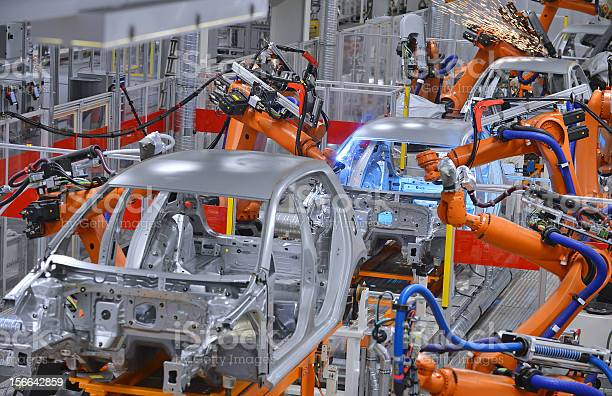
\includegraphics[width=8cm, keepaspectratio]{img/brazo}
    \caption{Brazo robótico.}
    \label{figura:brazo_robotico}
\end{figure}

En la actualidad, cada vez son más populares los coches autónomos. Es un campo muy amplio que cuenta con un gran número de posibilidades. Alguna de estas posibilidades serían los coches con conducción autónoma de \textit{Tesla}  (Figura 1.2) o los coches con aparcamiento autónomo que están desarrollando un gran número de compañías en la actualidad.

\begin{figure}[H]
	\centering
    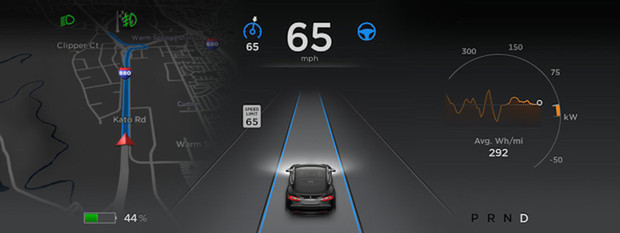
\includegraphics[width=8cm, keepaspectratio]{img/coche}
    \caption{Coche autónomo.}
    \label{figura:coche_autonomo}
\end{figure}

Otro campo de la aplicación de la robótica es la medicina, donde existen robots capaces de filtrar las vibraciones naturales del humano para proporcionarle una gran precisión y seguridad, un claro ejemplo es el robot DaVinci (Figura 1.3). Adicionalmente, hay robots capaces de mantener una estabilidad la estabilidad necesaria para caminar sobre dos piernas robóticas, como es el robot ATRIAS (Figura 1.4).

\begin{figure}[H]
  \centering
  \begin{minipage}[b]{0.4\textwidth}
    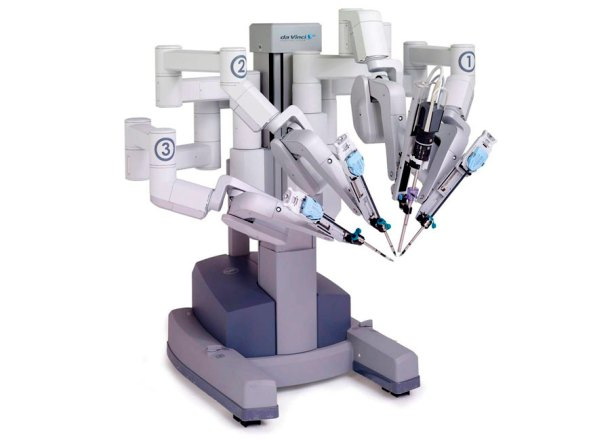
\includegraphics[width=\textwidth]{img/davinci}
    \caption{Robot DaVinci.}
    \label{figura:robot_davinci}
  \end{minipage}
  \hfill
  \begin{minipage}[b]{0.4\textwidth}
    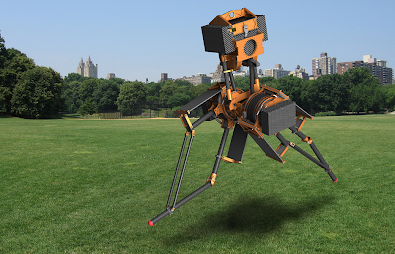
\includegraphics[width=\textwidth]{img/atrias}
    \caption{Robot ATRIAS.}
    \label{figura:robot_atrias}
  \end{minipage}
\end{figure}

En el ámbito militar, existen robots capaces de sustituir a una persona en el a la hora de realizar tareas de gran peligro como la desactivación de bombas y la entrada en zonas contaminadas (Figura 1.5).

\begin{figure}[H]
	\centering
    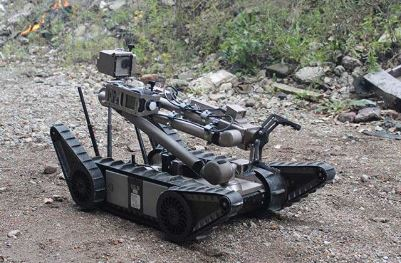
\includegraphics[width=8cm]{img/robot_militar}
    \caption{Robot militar.}
    \label{figura:coche_autonomo}
\end{figure}

\section{Componentes robóticas}
\label{subsec:componentes roboticas}

Todo robot está formado por dos componentes: el \textit{software}, encargado de proporcionar la inteligencia al robot, el más importante, y, el \textit{hardware} encargado de proporcionar la estructura física del robot.

Con al gran auge de la robótica han surgido numerosas plataformas que proporcionan herramientas que simplifican el desarrollo de software robótico, esto son los denominados \textit{middlewares} robóticos.

Durante el desarrollo de software robótico es preciso realizar una serie de pruebas para comprobar el funcionamiento del código y depurar errores, por lo que se necesitan simuladores que nos proporcionen un entorno cercano a la realidad previa al ensamblado del robot.

\subsection{Middlewares robóticos}
\label{subsec:middlewares}

Un \textit{middleware} robótico es un \textit{framework} que proporciona una serie de herramientas que facilitan el desarrollo de software para robots. Proporciona los servicios necesarios para soportar y simplificar aplicaciones complejas y distribuidas. Para el control de los sensores y actuadores de los robots, los \textit{middlewares} proporcionan \textit{drivers}, APIs, etc.

\emph{OpenRDK} es un proyecto de código abierto para el desarrollo de módulos poco acoplados. Proporciona una gestión de concurrencia, comunicación entre procesos y una técnica de enlace que permite el diseño de sistemas conceptuales de puertos de datos de entrada / salida. También proporciona módulos para realizar conexiones con simuladores robóticos y controladores de robots genéricos. También existen algunos otros \emph{middlewares} como \emph{Micro} y \emph{Orca}.

El \textit{middleware} robótico más generalizado es ROS\footnote{\url{https://www.ros.org/}}
 (\textit{Robotics Operating System}). \textit{Robotics Operating System} fue desarrollado en 2007 por el Laboratorio de Inteligencia Artificial de Stanford para dar soporte a sus proyectos. A pesar de no ser un sistema operativo, ROS proporciona servicios como la abstracción \textit{hardware}, mecanismos de comunicación entre prosesos, el control de dispositivos de bajo nivel y el mantenimiento de paquetes. \textit{Robotics Operating System} fue desarrollado para sistemas UNIX, aunque en la actualidad está siendo adaptado para su funcionamiento en sistemas operativos como Fedora, Mac OS X, Arch, Gentoo, OpenSUSE, Slackware, Debian o Microsoft Windows.

\subsection{Simuladores robóticos}
\label{subsec:simuladores}

Los simuladores robóticos surgen con la necesidad de realizar pruebas durante el desarrollo del \textit{software} para la detección y depuración de posibles errores antes de llevarlo a un robot real debido al gran coste que suponen.

Uno de los simuladores más utilizados en la actualidad es \textit{Gazebo}\footnote{\url{http://gazebosim.org/}}. Su popularidad se debe a su robusto motor de físicas, sus gráficos de alta calidad y su amplio catálogo de robots y escenarios. Es una herramienta de código abierto integrada con ROS, por lo que permite ejecutar \textit{software} robótico en un escenario simulado (Figura 1.6).

\begin{figure}[H]
	\centering
    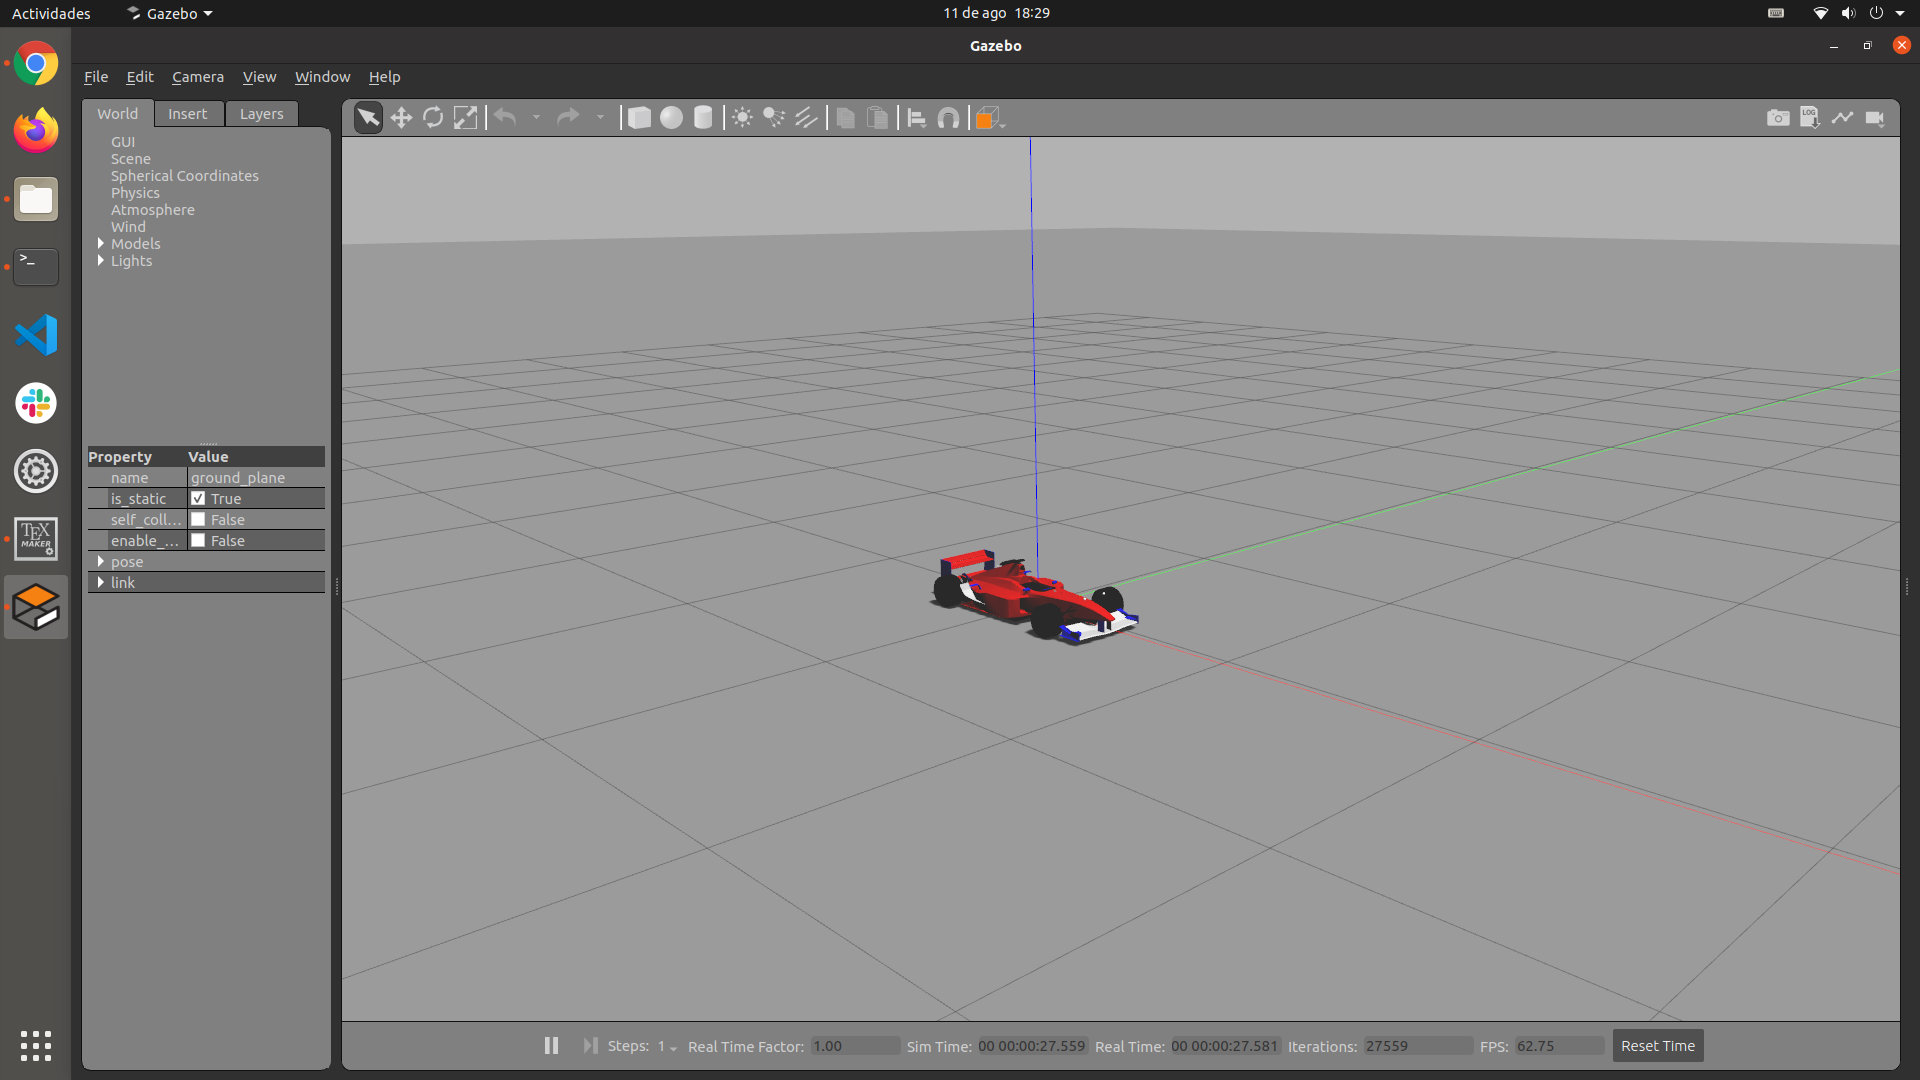
\includegraphics[width=\textwidth]{img/gazebo}
    \caption{Simulador Gazebo.}
    \label{figura:simulador_gazebo}
\end{figure}

\section{Robótica educativa}
\label{sec:robotica educativa}

La robótica educativa proporciona a los estudiantes la infraestructura para la construcción y programación de un robot, pero, además de la enseñanza robótica,
estos entornos van más allá, ofrenciendo la capacidad para el alumno de adquirir un pensamiento lógico. También, contribuye en la adquisición de una mentalidad resolutiva y al enriquecimiento de la cultura científica de los alumnos. Este método de educación con la robótica como objeto de enseñanza se denomina el método STEAM (Science, Technology, Engineering, Arts and Matemathics).

Como se ha comentado, para llevar a cabo este método de educación es necesaria una infraestructura, como alguna plataforma cuyo objetivo sea el de la enseñanza de la robótica, algunas de estas plataformas son las siguientes:

\begin{itemize}
\item \textbf{Robocode:} es un juego de programación en \emph{Java} o \emph{.NET}, cuyo objetivo es programar la lógica de un robot que es un tanque de batalla, para combatir contra otros tanques. Esta plataforma ofrece una comunidad que incluye uuna Wiki y un grupo de google. Además, ha realizado una competición propia \footnote{\url{https://gamesfleadh.ie/robocode/}}.
\item \textbf{CodeCombat:} ofrece un aprendizaje basado en juegos, tiene el objetivo de que los estudiantes aprendan mientras juegan. Los estudiantes aprenderán \emph{JavaScript}, \emph{Python}, \emph{HTML} y \emph{CoffeeScript}, además de aprender los fundamentos de la informática. El contenido se divide en 11 unidades: tres unidades de desarrollo de juegos, dos unidades de desarrollo web y seis unidades de informática.
\item \textbf{Gearsbot:} un entorno de programación de robots mediante bloques, que además también ofrece la posibilidad de programar la lógica en \emph{Python}, usa un simulador web que emplea la tecnología \emph{WebGL} \footnote{\url{https://es.wikipedia.org/wiki/WebGL}} para renderizar gráficos.
\item \textbf{Riders.ai:} una plataforma de programación de robots que ofrece la posibilidad de realizar competiciones idividuales como en grupos. Es accesible desde cualquier lado del mundo. También ofrece al usuario una capa de abstracción sobre los sensores, localización y diferentes partes del robot.
\item \textbf{TheConstruct:} ofrece un entorno de programación de robots que pueden moverse por la Luna, Marte y más planetas. No requiere la instalación de ROS. Ofrece un gran extra que le diferencia de los demás, esto es, brinda la posibilidad al usuario de poder ejecutar su código en robots reales de forma remota, y, también proveen certificados al completar diferentes cursos.
\end{itemize}

Dentro de la robótica educativa, es preciso enfatizar la plataforma \textit{Unibotics} en la que se desarrolla el presente proyecto. Esta plataforma es un proyecto internacional que ofrece material para la enseñanza de robótica en las aulas. \textit{Unibotics} proporciona una infraestructura software en conjunto a una colección de ejercicios, cada uno con el material teórico correspondiente para su resolución.

\subsection{Tecnologías Web}

Las diferentes tecnologías web permiten crear interfaces de usuario y establecer las comunicaciones con el servidor, además de implementar comportamientos de la web en el servidor. Se pueden distinguir en tecnologías \emph{backend} (del lado del servidor) y tecnologías \emph{frontend} (del lado del usuario).

Una gran ventaja de estas tecnologías es que ofrecen la ausencia de la necesidad de instalar componentes de software, configuración y dependencias adicionales. Únicamente es necesario disponer de un navegador de internet y una conexión a internet, pues todos los archivos necesarios se servirán desde el lado del servidor.

Estas tecnologías facilitan el uso al cliente, pues evitan que el usuario tenga que intalar actualizaciones, pues las actualizaciones se realizan en el lado del servidor. Esta ventaja elimina posibles fallos debidos a incompatibilidades entre las versiones, pues el servidor distribuye una única version para todos. También ofrecen la ventaja de aplicaciones web multiplataforma, únicamente es necesario el desarrollo en un único entorno (\emph{Windows}, \emph{Ubuntu}, \emph{MacOS}, etc), pues estas tecnologías son comunes a los navegadores de todos los sistemas. Únicamente es necesario conocer \emph{HTML}, \emph{CSS} y \emph{JavaScript}, el navegador será el encargado de interpretar dichos lenguajes.

Las aplicaciones web dependen de una conexión entre el usuario y el servidor, por lo que, una de las desventajas que estas es la latencia que esta conexión pueda generar. Estas tecnologías siempre son algo más lentas que otros lenguajes compilados como \emph{C\#} puesto que el navegador no realiza ninguna compilación, si no que interpreta el código línea a línea.

En el lado del servidor, existen diversos \emph{frameworks} que facilitan la vida al desarrollador. Algunos ejemplos de ellos serían, \emph{Express} para el lenguaje \emph{JavaScript} y \emph{Django} escrito en \emph{Python}.

El desarrollo de tecnologías web está sujeto a un gran crecimiento. Cada vez las aplicaciones web son más potentes y eficientes, de manera que cada vez son más los desarrolladores que optan por este modelo de desarrollo.

Las tecnologías web ofrecen la posibilidad de que varios usuarios puedan programar robots y ejecutarlos en el mismo escenario, hacer competiciones tanto síncronas como asíncronas, algo que resultaría muy complejo si se realizase en local. \emph{WebRTC} nos ofrece esta posibilidad, pues es una herramienta de código abierto que proporciona conexiones en tiempo real entre \emph{peers} mediante un API.

\subsection{Estructura del documento}

En esta sección se va a hacer un breve resúmen de los contenidos de cada capítulo, también se mencionará como están estructurados.

En el capítulo 2, Objetivos, se explica cuál es el propósito o los propósitos de este trabajo. También se mencionará la planificación temporal que se ha llevado a cabo durante el trabajo. Y finalmente, se mencionará la heramienta empleada para realizar un control de versiones.

Posteriormente, en el capítulo 3, Herramientas, se habla exclusivamente sobre las herramientas y tecnologías utilizadas. Serán descritas indicando sus ventajas, inconvenientes y áreas de uso.

A continuación, en el capítulo 4, Juegos Asíncronos, se explicará cómo se ha realizado el diseño de los mismos, tanto para la IU como para la infraestructura interna.

Seguidamente, en el capítulo 5, Juegos Síncronos, de igual manera que en la sección anterior, se explicará como se ha desarrollado la infraestructura necesaria para elaborar el ejercicio.

Finalmente, en el capítulo 6, tenemos los experimentos realizados y sus resultados, además, en el capítulo 7, se encuentran las conclusiones obtenidas de haber realizado este trabajo, y, en último lugar la bibliografía que contiene todos los contenidos empleados para el desarrollo del trabajo.

%%%%%%%%%%%%%%%%%%%%%%%%%%%%%%%%%%%%%%%%%%%%%%%%%%%%%%%%%%%%%%%%%%%%%%%%%%%%%%%%
%%%%%%%%%%%%%%%%%%%%%%%%%%%%%%%%%%%%%%%%%%%%%%%%%%%%%%%%%%%%%%%%%%%%%%%%%%%%%%%%
% OBJETIVOS %
%%%%%%%%%%%%%%%%%%%%%%%%%%%%%%%%%%%%%%%%%%%%%%%%%%%%%%%%%%%%%%%%%%%%%%%%%%%%%%%%

\cleardoublepage % empezamos en página impar
\chapter{Objetivos} % título del capítulo (se muestra)
\label{chap:objetivos} % identificador del capítulo (no se muestra, es para poder referenciarlo)

En este capítulo se explicarán los objetivos que se pretenden alcanzar en este TFG, los requisitos para los problemas que se van a plantear, la planificación y metodología seguida durante todo el desarrollo.

\section{Objetivos} % título de sección (se muestra)
\label{sec:objetivo-general} % identificador de sección (no se muestra, es para poder referenciarla)

El objetivo general de este trabajo es la introducción de juegos en la plataforma \emph{Unibotics}, en los que varios usuarios puedan competir síncrona y asíncronamente para fomentar su aprendizaje. Este objetivo principal se ha dividido en dos subobjetivos.

\begin{itemize}
\item La introducción de \textbf{juegos competitivos asíncronos} que permitan a los usuarios competir contra una serie de dificultades proporcionadas por la plataforma, en el mismo escenario y en tiempo real.
\item La introducción de \textbf{juegos competitivos síncronos} que proporcionan una visión más competitiva y social de la plataforma a los usuarios, que pueden conectarse simultáneamente con sus amigos para competir entre ellos.
\end{itemize}

Las soluciones proporcionadas deben cumplir los objetivos previamente mencionados, además de los siguientes requisitos para una correcta implementación:

\begin{itemize}
\item El código del lado del servidor debe ser desarrollado en \emph{HTML}, \emph{CSS3} y \emph{JavaScript}.
\item No debe requerir instalaciones de software adicionales, el usuario unicamente ha de tener el contenedor docker \emph{RADI}, instalado en la máquina local.
\end{itemize}

\section{Metodología}
\label{sec:metodologia}

Para llevar a cabo este trabajo, se ha empleado una metodología basada en \emph{sprints} \footnote{\url{https://www.bbva.com/es/metodologia-scrum-que-es-un-sprint/}}. Este modelo de desarrollo se corresponde con un modelo de desarrollo de software ágil, consiste en dividir un proyecto en tareas más sencillas y de menor duración, de forma que cada cierto período de tiempo (1-2 semanas) puedan presentarse resultados. Esta metodología es muy útil pues, es susceptible a cambios por parte del cliente.

Para la implantación de esta metodología se han establecido reuniones semanales. En dichas reuniones se ha comentado los cambios que se han introducido en el \emph{sprint} previo para proponer cambios, mejoras y fijar una serie de objetivos para la siguiente semana.

%\section{Planificación temporal}
%\label{sec:planificacion-temporal} 

\section{Plan de trabajo}
\label{sec:plan-de-trabajo}

Para el seguimiento de los objetivos previamente mencionados, se ha seguido una serie de etapas que permiten el avance incremental en la implementación del trabajo.

\begin{itemize}
\item \textbf{Estudio de la plataforma Unibotics:} Como una primera toma de contacto es preciso el estudio de la infraestructura que se está empleando en la plataforma. Además, se ha realizado la puesta en funcionamiento del \emph{despliegue local} \footnote{Despliegue de un clon de la plataforma en un entorno local con el fin de realizar cambios y probar nuevas funcionalidades, previo a incorporar los cambios a la plataforma oficial}, el contenedor docker (\emph{RADI}) y la comprobación de que todos los ejercicios funcionan de manera correcta. También, se ha estudiadio el funcionamiento de las platillas empleadas por los ejercicios y la conexión con el \emph{RADI}.

\item \textbf{Desarrollo de los juegos asíncronos:} Una vez entendidos los conceptos pricipales de la plataforma, se ha procedido al desarrollo de los juegos asíncronos. Se han diseñado nuevas plantillas para los nuevos ejercicios asícronos, y, añadido nuevos aspectos, como evaluadores automáticos.

\item \textbf{Estudio de la tecnología WebRTC:} Una vez completada la parte de los juegos asíncronos, se procede al estudio de estas tecnologías que nos permiten la retransmision de audio y vídeo entre dos navegadores web. Se han desarrollado algunos pequeños programas de prueba, como un chat de texto y vídeo, para asentar los conceptos.

\item \textbf{Desarrollo del juego síncrono:} Con los conceptos de WebRTC asentados, se ha procedido a diseñar en el webserver de \emph{Unibotics}, un sistema de señalización entre los usuarios, de manera que se pueda intercambiar la información necesaria para realizar la conexión WebRTC. Finalmente, en las plantillas del ejercicio, se incluye código \emph{JavaScript} que se encarga de establecer las conexiones RTC para cada extremo.
\end{itemize}

%%%%%%%%%%%%%%%%%%%%%%%%%%%%%%%%%%%%%%%%%%%%%%%%%%%%%%%%%%%%%%%%%%%%%%%%%%%%%%%%
%%%%%%%%%%%%%%%%%%%%%%%%%%%%%%%%%%%%%%%%%%%%%%%%%%%%%%%%%%%%%%%%%%%%%%%%%%%%%%%%
% HERRAMIENTAS %
%%%%%%%%%%%%%%%%%%%%%%%%%%%%%%%%%%%%%%%%%%%%%%%%%%%%%%%%%%%%%%%%%%%%%%%%%%%%%%%%

\cleardoublepage % empezamos en página impar
\chapter{Herramientas} 
\label{chap:herramientas}

En este capítulo se hará una breve presentación de todas las herramientas empleadas para el desarrollo del presente TFG. Estas tecnologías se pueden englobar en dos grupos, las tecnologías Front-End dedicadas a la presentación y a la interfaz de usuario (JavaScript, HTML y CSS), tecnologías Back-End dedicadas al servidor (Django), y, por último, tecnologías WebRTC que serán las encargadas de transmitir el vídeo en los juegos síncronos. 

\section{Lenguaje JavaScript}
\label{sec:javascript}

Se trata de un lenguaje de programación interpretado, su estándar es \textit{ECMAScript}\footnote{Especificación de lenguaje de programeción que define un leguaje de tipos dinámicos y soporta programación orientada a objetos basada en prototipos.}, basado en \textit{Java} y \textit{C}. Fue creado para aplicaciones web del lado del cliente. Es interpretado en el navegador web y permite mejoras en la interfaz de usuario, además de páginas web dinámicas. Tembién puede usarse en el lado del servidor utilizando \textit{Node.js}, un entorno de ejecucción de JavaScript construido con el motor \textit{JavaScript V8}.

En este proyecto se ha empleado JavaScript en el lado del cliente. La lógica de las plantillas que usan los ejercicios ha sido programada usando \textit{ECMAScript-6}, así como los evaluadores automáticos de los mismos, y, adicionalmente, para los \textit{WebSockets} encargados de comunicarse con el servidor para realizar tareas de señalización, o de envío de mensajes. Sus principales características son:

\subsection{Caractrerísticas del lenguaje}
\label{subsec:javascript}

\begin{itemize}
	\item Se trata de un lenguaje del lado del cliente, es decir, ejecuta en la máquina del propio cliente a través de un navegador.
	
	\item Tipado débil, por lo que no es necesario especificar el tipo de dato al declarar una variable permitiendo que una misma variable pueda adquirir distintos tipos durante la ejecucción.
	
	\item De alto nivel, con lo que significa que su sintaxis es fácilmente comprensible. Esta sintaxis se encuentra alejada del lenguaje máquina.
	
	\item Es un lenguaje interpretado puesto que utiliza un intérprete que traduce las líneas de código a lenguaje máquina en tiempo de ejecucción.

	\item Es un leguaje orientado a objetos, ya que utiliza clases y objetos como estructuras.
\end{itemize}

Adicionalmente, junto con \textit{ES-6} se ha empleado una librería llamada \textit{jQuery}\footnote{\url{https://jquery.com/}} que permite agregar dinamismo a un sitio web permitiendo interactuar con los elementos HTML, manipular el DOM, manejar eventos, diseñar animaciones y agregar interacción con la técnica \textit{AJAX}\footnote{\url{https://developer.mozilla.org/es/docs/Web/Guide/AJAX}} (\textit{Asynchronous JavaScript and XML}).

\subsection{Librería jQuery}
\label{subsec:javascript}

\textit{jQuery} es una librería multiplataforma desarrollada en JavaScript, inicalmente desarrollada por John Resig. Esta librería permite simplificar en gran medida la interacción con los documentos HTML y sus estilos, manipular el DOM, manejar eventos, crear animaciones, y agregar la integración de la técnica \textit{AJAX} (\textit{Asynchronous JavaScript and XML}).

En código, el constructor de jQuery puede llamarse empleando el nombre \textit{jQuery}, o, también empleando el alias \textit{\$}.

Esta librería hace posible a desarrolladores que se inician en el mundo del desarrollo de interfaces de aplicación, puedan desarrollar una interfaz gráfica más elaborada sin la necesidad de tener amplios conocimientos de CSS.

\section{Lenguaje HTML}

\textit{HTML} (\textit{HyperText Markup Languaje}) es un lenguaje de marcado que permite indicar la estructura un documento utilizando etiquetas. Es utilizado para la creación de documentos electrónicos que se envían a través de la red. Los documentos pueden tener conexiones con otros a través de \textit{hipervínculos}.

\begin{figure}[H]
	\centering
    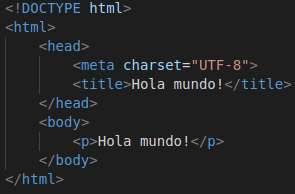
\includegraphics[width=8cm]{img/html}
    \caption{Documento básico de \textit{HTML}.}
    \label{figura:simulador_gazebo}
\end{figure}

Primeramente se debe declarar el tipo del documento \textit{HTML} mediante la línea \textit{DOCTYPE html} que indica que es un documento \textit{HTML-5}. El elemento \textit{html} engloba el documento \textit{HTML}, dentro de este elemento se encuentran dos etiquetas:

\begin{itemize}
	\item \textit{HEAD} es la cabecera del documento, que contiene la información general (metadatos) acerca del documento, incluyendo el título y los enlaces a scritps y hojas de estilos.
	
	\item \textit{BODY} es el cuerpo del documento \textit{HTML} donde se encuentran las etiquetas que dan formato al mismo. Puede contener imágenes, enlaces, vídeos, menús, formularios, botones, además de animaciones, que se pueden crear dentro de un elemento canvas.
\end{itemize}

Con la incorporación de \textit{HTML-5} se han introducido diversas novedades y mejoras que son de interés para este trabajo:

\begin{itemize}
	\item \textit{WebSockets}, es una tecnología que hace posible abrir una comunicación entre el navegador y el servidor.
	
	\item \textit{WebRTC} (\textit{Web Real-Time Communications}) es una tecnología que permite a las aplicaciones web capturar y transmitir audio y vídeo entre navegadores sin necesidad de un intermediario.
	
	\item Se añade un mejor soporte de contenido multimedia sin la necesidad de instalar plugins adicionales. Mediante el elemento \textit{video} la página reproducirá de manera nativa el contenido.
	
	\item Proporciona un elemento, \textit{canvas} que permite renderizar escenas gráficas en la web mediante el uso de \textit{JavaScript}.
\end{itemize}

\section{Hojas de estilo CSS}
\label{sec:css}

CSS o \textit{Cascading Stylesheet} es un lenguaje empleado para dar formato y estilo a un documento de texto, comunmente, las instrucciones se agrupan en archivos con extensión \textbf{*.css}, lo que permite que para una página web se puedan almacenar estilos por separados dependiendo del fin de cada uno, de esta manera, se podrán importar en cada documento únicamente las instrucciones de las que se va a hacer uso.

Con respecto a lo último mencionado, puesto que estas hojas almacenan el estilo, CSS nos ofrece una gran ventaja, la separación de la estructura del documento (HTML) de su representación. Aunque es posible añadir instrucciones CSS en el \textit{head} de un documento HTML mediante la etiqueta \textit{style}, esto no es una buena práctica.

\textit{Cascading Stylesheet} nos permite utilizar \textit{JavaScript} para si fin principal, el de dar dinamismo e inteligencia a una página web, etc. Por lo que mejora en gran manera el rendimiento de la página.

A continuación se muestra un ejemplo del uso de este lenguaje.

\begin{figure}[H]
	\centering
    
\includegraphics[width=15cm]{img/nocss_vs_css}
    \caption{Comparativa entre no usar CSS y usarlo.}
    \label{figura:nocss_vs_css}
\end{figure}

Como se puede apreciar en la imagen 3.2, hay un gran salto de no usar CSS a usarlo en los documentos HTML. Este lenguaje nos permite tamto crear un \textit{Navbar}, menús desplegables, barras de búsqueda, botones personalizados, sub-apartados, es decir, aumenta en gran medida la experiencia del usuario.

CSS también permite la creación de páginas web responsivas, esto es, que la web se adapte al tamaño de la pantalla del usuario, redimensionando los elementos y recolocándolos. Esto es muy útil si se quiere desarrollar una aplicación multiplataforma.

\section{Django para servidores web}
\label{sec:django}

Django \footnote{\url{https://es.wikipedia.org/wiki/Django_(framework)}} \cite{django} es un framework de alto nivel que facilita el desarrollo de sitios web seguros y sostenibles. Fue lanzado como un framework web genérico en 2005, bajo una licencia de código abierto. Django se encarga de las complicaciones del desarrollo web, para que el usuario pueda centrarse en escribir su aplicación.

El objetivo de Django es la creación sencilla de sitios web complejos, poniendo énfasis en la reutilización, la conectividad y la extensibilidad de componentes, el desarrollo rápido y el principio de no repetir código (\textit{Don't Repeat Yourself}).

Algunas de las carácterística de Django son:

\begin{itemize}
\item Un mapeador objeto-relacional, es capaz de convertir datos entre un sistema de tipos utilizado en un lenguaje de programación orientado a objetos y la utilización de una base de datos relacional.

\item Aplicaciones incorporables en cualquier página gestionada con Django.

\item Una API de base de datos robusta.

\item Un sistema incorporado de "vistas genéricas" que ahorra el tener que escribir la lógica de ciertas tareras comunes.

\item Un sistema extensible de plantillas con herencia.

\item Un despachador de URLs basado en expresiones regulares.

\item Un sistema \textit{middleware} para desarrollar caracteríscas adicionales.

\item Soporte de internacionalización, incluyendo traducciones de la interfaz de administración.

\item Documentación incorporada accesible a través de la aplicación administrativa.
\end{itemize}

\section{WebRTC}
\label{sec:webrtc}

WebRTC \footnote{\url{https://es.wikipedia.org/wiki/WebRTC}} \cite{webrtc} (Web Real-Time Communication) es un proyecto libre y de código abierto que proporciona una comunicación en tiempo real (RTC) a través de una serie de APIs. Permite que la comunicación de audio y vídeo funcione dentro de las páginas web al permitir la comunicación \textit{Peer to Peer}, sin necesidad de instalación de plugins y sin necesidad de la intervención del servidor. WebRTC tiene soporte en los navegadores Safari, Chrome, Firefox, Mozilla y Opera, está estandarizado por el World Wide Web Consortium \footnote{\url{https://es.wikipedia.org/wiki/World_Wide_Web_Consortium}} y por el Internet Engineering Task Force \footnote{\url{https://es.wikipedia.org/wiki/Grupo_de_Trabajo_de_Ingenier\%C3\%ADa_de_Internet}}.

El API de WebRTC tiene una serie de interfaces principales que son clave en el dearrollo del software para este proyecto:

\begin{itemize}
\item \textbf{RTCPeerConnection} \footnote{\url{https://developer.mozilla.org/es/docs/Web/API/RTCPeerConnection}} representa una conexiñon entre una máquina local y un par remoto. Esta interfaz provee métodos para: conectar un equipo remoto, mantener y monitorizar esa conexión y cerrar la conexión.

\item \textbf{RTCDataChannel} \footnote{\url{https://developer.mozilla.org/en-US/docs/Web/API/RTCDataChannel}} representa el canal que puede ser empleado para la transmisión de datos \textit{Peer to Peer}.

\item \textbf{MediaDevices} \footnote{\url{https://developer.mozilla.org/es/docs/Web/API/MediaDevices}} proporciona el acceso a los dispositivos multimedia conectados, como webcams y micrófonos, y, también para compartir la pantalla. Ofrece un método \textit{getUserMedia()}, que, con el permiso del usuario, enciende la cámara, obtiene la imagen de la pantalla, el audio del micrófono, y, proporciona un \textit{MediaStream} que contiene pistas de vídeo y/o de audio del dispositivo.

\item \textbf{MediaStream} \footnote{\url{https://developer.mozilla.org/en-US/docs/Web/API/MediaStream}} representa el flujo de contenido multimedia. Un flujo consiste de varias pistas, ya sean de audio o de vídeo.
\end{itemize}

\subsection{Protocolos}
\label{subsec:protocolos}

\begin{itemize}
\item \textbf{ICE} \footnote{\url{https://en.wikipedia.org/wiki/Interactive_Connectivity_Establishment}} (\textit{Interactive Conectivity Establishment}). Es una técnica empleada para permitir que un navegador web se conecte con otro/s navegador/es web mediante conexiones \textit{Peer to Peer}. Debe de poder pasar por un \textit{firewall}, dirección IP pública, y, transmitir los datos a través de otro servidor, si el \textit{router} no permite las conexiones entre pares. Para lograr esta serie de casos, se emplean servidores STUN y TURN.


\item \textbf{STUN} \footnote{\url{https://en.wikipedia.org/wiki/STUN}} (\textit{Session Transvelsal Utilities for NAT}). Es un protocolo de descubrimiento de IP pública, para determinar cualquier restricción en el \textit{enrutador} que impida una conexión directa con un par. El cliente enviará una solicitud STUN en Internet que responderá con la dirección pñublica del cliente y si el cliente esta accesible detrás del NAT del enrutador.

\item \textbf{NAT} \footnote{\url{https://en.wikipedia.org/wiki/Nat}} (\textit{Network Address Translation}). Es empleado por el \textit{router} para asignar una dirección IP pública. El \textit{router} tiene acceso a la dirección pública de cada dispositivo y cada dispositivo conectado a este, tendrá una dirección IP privada. Las solucitudes se traducen de la IP privada a la IP pública con un puerto único. Algunos \textit{enrutadores} tienen restricciones sobre quien puede conectarse a su red. Esto puede dar lugar a que aunque tengamos un única dirección IP pública encontrada por el servidor STUN, no se pueda establecer una conexión. Ante este caso, se debe recurrir a un servidor TURN.

\item \textbf{TURN} \footnote{\url{https://en.wikipedia.org/wiki/Traversal_Using_Relays_around_NAT}} (\textit{Transversal Using Relays around NAT}). Algunos router emplean una técnica llamada \textit{NAT simétrica}. Esto es, el \textit{enrutador} solo acepta conexiones de pares a los que se haya conectado previamente. TURN está destinado a aludir esta resticción de NAT simétrica. Consiste en establecer una conexión con un servidor TURN que retransmite todo el tráfico que se le envía, de una máquina a otra. Este intercambio es gestionado usando ICE.

El proceso de \textit{Offer}/\textit{Answer} es realizado cuando se establece una nueva conexión, o bien, cuando debe cambiar un aspecto de una conexión ya establecida. A continuación se enumeran los pasos que ocurren durante el intercambio de la oferta y la respuesta:


\begin{figure}[H]
  \centering
  \begin{minipage}[b]{0.4\textwidth}
    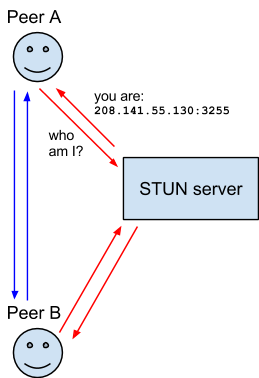
\includegraphics[width=\textwidth,height=60mm]{img/stun.png}
    \caption{Protocolo STUN.}
    \label{figura:stun}
  \end{minipage}
  \hfill
  \begin{minipage}[b]{0.4\textwidth}
    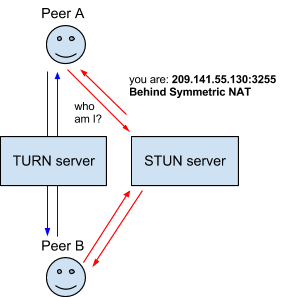
\includegraphics[width=\textwidth,height=60mm]{img/turn.png}
    \caption{Protocolo TURN.}
    \label{figura:turn}
  \end{minipage}
\end{figure}

\item \textbf{SDP} (\textit{Session Description Protocol}) \footnote{\url{https://en.wikipedia.org/wiki/Session_Description_Protocol}}. Es un protocolo empleado para describir el contenido multimedia de una conexión.

\end{itemize}

\subsection{Establecimiento de la conexión}
\label{subsec:establecimiento_conexion}

El protocolo WebRTC se encarga de establecer conexiones entre pares, pero desafortunadamente, una conexión WebRTC no se puede establecer sin un servidor intermedio. Este servidor podríamos llamarlo \textbf{servidor de señalización}, empleado en el intercambio de información previo al establecimiento de la conexión WebRTC.

La información que necesitamos intercambiar es una \textit{Offer} y una \textit{Answer} que contienen el \textit{Session Description Protocol} mencionado anteriormente en \ref{subsec:protocolos}.

El \textit{Peer A} que inicia la conexión va a crear una oferta (\textit{Offer}). Esta \textit{Offer} será enviada al \textit{Peer B} mediante el servidor intermedio seleccionado. \textit{Peer B} recibirá esta \textit{Offer} desde el servidor de señalización y creará una respuesta (\textit{Answer}) que enviará haciendo uso del mismo intermediario al \textit{Peer A}.

\begin{enumerate}
\item \textit{Peer A} captura los medios locales mediante \textit{MediaDevices.getUserMedia}

\item \textit{Peer A} crea una conexión \textit{RTCPeerConnection} y emplea el método \textit{RTCPeerConnection.addTrack()} para añadir el flujo de datos a la comunicación.

\item \textit{Peer A} crea la \textit{Offer} mediante el método \textit{RTCPeerConnection.createOffer()}.

\item \textit{Peer A} establece el SDP de su \textit{Offer} llamando al método \textit{RTCPeerConnection.setLocalDescription()}.

\item \textit{Peer A} solicita al servidor STUN que genere los candidatos ICE.

\item \textit{Peer A} usa el servidor de señalización para transmitir su \textit{Offer}.

\item \textit{Peer B} recibe la oferta y emplea \textit{RTCPeerConnection.setRemoteDescription()} para almacenar el SDP de \textit{Peer A}.

\item \textit{Peer B} hace la configuración necesaria relativa a su conexión, como obtener su flujo de datos multimedia.

\item \textit{Peer B} crea una respuesta haciendo uso del método \textit{RTCPeerConnection.createAnswer()}.

\item \textit{Peer B} establece su descripción local llamando a \textit{RTCPeerConnection.setLocalDescription()} y pasando la respuesta por parámetro.

\item \textit{Peer B} envía la respuesta usando el servidor de señalización.

\item \textit{Peer A} recibe \textit{Answer}.

\item \textit{Peer A} almacena el SDP de \textit{Peer B} llamando al método \textit{RTCPeerConnection.setRemoteDescription()}. Ahora \textit{Peer A} y \textit{Peer B} tienen la configuración de ambos y el flujo de medios comienza a transmitirse.
\end{enumerate}

\subsection{Candidatos ICE}
\label{subsec:candidatos_ice}

Además de intercambiarse la información sobre los elementos multimedia, los \textit{peers} deben intercambiar información sobre la conexión. Esto es conocido como \textit{candidatos ICE}, que detallan los métodos disponibles con los que un extremo puede comunicarse (directamente o mediante un servidor TURN). Cada \textit{peer} propondra una lista con sus mejores candidatos primero, estos candidatos son UDP (puesto que es más rápido, pues no hay retransmisiones, ni recuperación frente a pérdidas), aunque también permite emplear candidatos TCP. Esta comunicación es transparente para el usuario.

\begin{figure}[H]
	\centering
    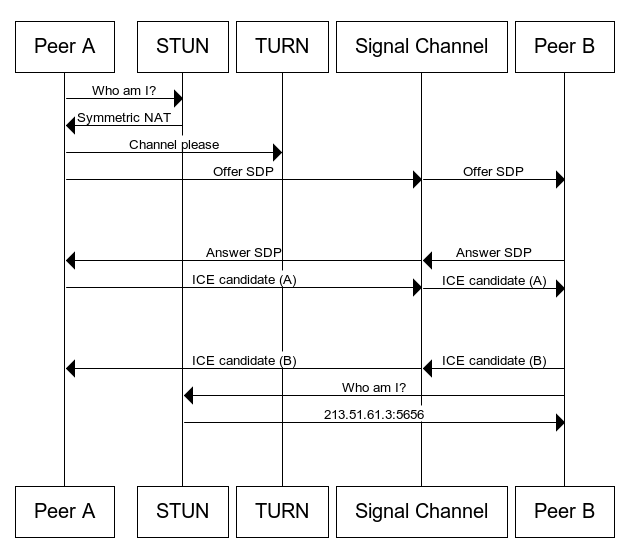
\includegraphics[width=10cm]{img/ice_diagram.png}
    \caption{Diagrama de intercambio de candidados ICE.}
    \label{figura:nocss_vs_css}
\end{figure}

\section{Control de versiones}
\label{sec:control-de-versiones}

En todo desarrollo de software es necesaria una herramienta de control de versiones que facilite la gestión del código fuente. Estos softwares realizan un control de todas las modificaciones, de manera que si se comete un error en un determinado instante, se puede volver a una versión anterior del código. La herramienta empleada para el control de versiones en este proyecto es \emph{GitHub}.

Esta herramienta permite clonar cualquier repositorio en nuestra máquina local y mantenerlo actualizado frente a cambios que se hagan en el extremo remoto. También podemos contribuir en este código realizando \emph{pull requests}. Es una herramienta muy potente, lo que le hace ser una de las herramientas de control de versiones más utilizadas por la comunidad de desarrolladores.

\emph{GitHub} proporciona un interfaz gráfico que nos permite, de manera gráfica, ver la actividad de un repositorio, lo que nos permite saber si un proyecto tiene una gran cantidad de desarrolladores.

\begin{figure}[H]
	\centering
    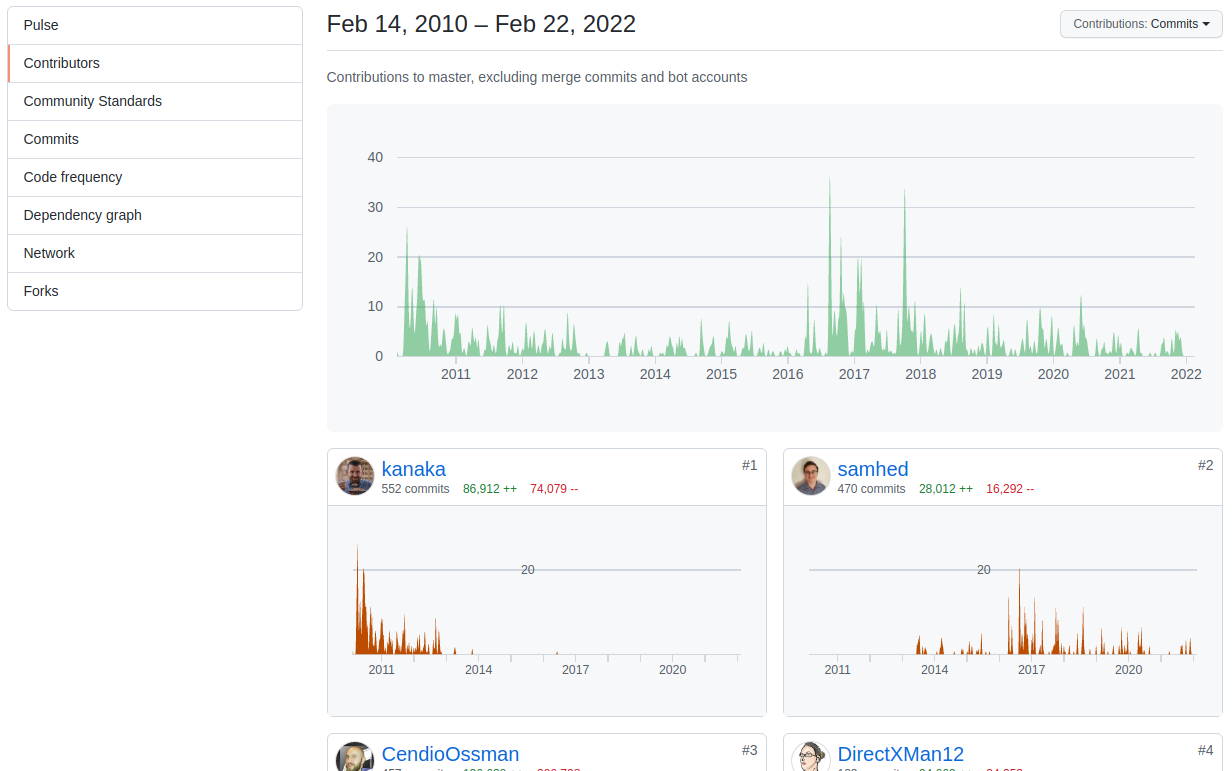
\includegraphics[width=15cm]{img/github_contributors.png}
    \caption{Gráfico de.actividad del repositorio \emph{noVNC} de GitHub.}
    \label{figura:simulador_gazebo}
\end{figure}

En este proyecto se ha trabajado en una serie de repositorios diferentes:

\begin{itemize}
\item \textbf{unibotics-webserver:} aquí se encuentran los recursos del webserver Django.
\item \textbf{unibotics-exercises:} este repositorio contiene las platillas de los ejercicios de la plataforma.
\item \textbf{RoboticsAcademy:} este repositorio es una colección \emph{open-source} de algunos retos, que se han empleado para diseñar ejercicios para la plataforma de \emph{Unibotics}.
\item \textbf{CustomRobots:} este repositorio contiene todos los robots empleados en las simulaciones.
\item \textbf{noVNC:} se ha realizado un \emph{fork} del repositorio oficial puesto que para la versión del ejercició síncrono se necesitaba hacer algunas modificaciones para enviar el flujo de vídeo al extremo remoto.
\end{itemize}

La metodología que se ha seguido para incorporar nuevos cambios a los disferentes repositorios es la siguiente. En primer lugar se crea una \emph{issue} el el repositorio correspondiente que describa el problema que se va a resolver. A continuación, se crea una rama a partir de la \emph{master} con el nombre de \emph{issue-XXX} donde se incorporarán todos los cambios mencionados en la \emph{issue} que se creó. Finalmente, una vez se han realizado todos los cambios y se ha verificado que funciona de manera correcta, se realiza un \emph{pull request}, esto es, una solicitud de incorporación de los cambios a la rama principal. Las \emph{pull request} son revisadas por otro compañero, que se encargará de hacer la pruebas pertinentes e incorporarla a la rama \emph{master}.

%%%%%%%%%%%%%%%%%%%%%%%%%%%%%%%%%%%%%%%%%%%%%%%%%%%%%%%%%%%%%%%%%%%%%%%%%%%%%%%%
%%%%%%%%%%%%%%%%%%%%%%%%%%%%%%%%%%%%%%%%%%%%%%%%%%%%%%%%%%%%%%%%%%%%%%%%%%%%%%%%
% JUEGOS ASÍNCRONOS %
%%%%%%%%%%%%%%%%%%%%%%%%%%%%%%%%%%%%%%%%%%%%%%%%%%%%%%%%%%%%%%%%%%%%%%%%%%%%%%%%

\cleardoublepage
\chapter{Juegos Asíncronos}

En este capítulo se expondrán los \emph{juegos asícronos} desarrollados para la plataforma de \textit{Unibotics}. Se han desarrollado un total de dos juegos asíncronos, de los que se hablará desde el diseño de las plantillas de la interfaz de usuario, hasta la comunicación con el servidor y el contenedor docker donde es ejecutado el juego. Para llevar a cabo el desarrollo de estos juegos, se ha partido de las versiones ya existentes dentro de la plataforma llamados \emph{retos}.

\section{Infraestructura}
\label{sec:async_infraestructura}

Para la realización de los siguientes ejercicios, trabajado sobre la infraestructura inicial sobre la que opera Unibotics. Esta arquitectura es formada por tres componentes, un \emph{Webserver}, el \emph{navegador} del usuario y el \emph{RADI} (contenedor Docker donde se ejecutan los ejercicios). A continuación, una descripción del trabajo que realiza cada componente:

\begin{itemize}
\item \textbf{Webserver:} este componente se encarga de proporcionar al navegador del usuario, los componentes del \emph{Front End} que van a ser  necesarios para llevar a cabo la ejecución del ejercicio en cuestión. Proporciona las plantillas \textbf{HTML} y el código \textbf{JavaScript}. También se encarga de almacenar y traer el código del usuario desde \textbf{AWS} (\emph{Amazon Web Services} \footnote{\url{https://es.wikipedia.org/wiki/Amazon_Web_Services}}), con el fin de tener una persistencia del código del mismo.

\item \textbf{Navegador:} ejecuta en la máquina del usuario, es el encargado de comunicarse con el RADI y mostrar toda la información relacionada con la simulación al usuario. Este componente muestra las plantillas de los ejercicios recibidas desde el Webserver al usuario. Mediante \emph{listeners} (escritos en \textbf{JavaScript}) sobre distintos elementos de la plantilla proporciona los controles sobre la ejecución del ejercicio (Play, Reset, Load Code, Gazebo, etc.). Además de proporcionar los controles sobre el ejercicio, también debe de transmitir estas órdenes al contenedor donde se aloja el ejercicio, de manera que durante el establecimiento de la conexión con este, en el caso de los juegos con dos vehículos, se establecen cinco WebSockets. Estos son, un máster, por el que se envían los comandos relacionados con el lanzamiento del ejercicio y Gazebo, y un dos WebSockets por cada vehículo, el primero \emph{ws\_code}, empleado para el envío del código al contenedor, se encarga de interactuar con el cerebro del robot, y, por útlimo, \emph{ws\_gui} cuya función es mostrar toda la información relativa a la interfaz de usuario (mapa al estilo f1, autoevaluador, imágenes de las cámaras), es decir, recibe toda la información del robot.

\item \textbf{RADI:} es uno de los componentes con más peso, pues es donde se ejecuta la simulación. Este ofrece una serie de elementos,  \emph{ws\_manager}, \emph{ws\_code} y \emph{ws\_gui} mencionados anteriormentes, y adicionalmente, ofrece la visualización de Gazebo mediante \emph{GZClient \footnote{\url{http://manpages.ubuntu.com/manpages/bionic/man1/gzclient.1.html}}} y de la consola del contenedor, ambos por medio de un servidor \emph{noVNC \footnote{\url{https://novnc.com/info.html}}} alojado localmente en el contenedor, al cual se conectará el navegador para mostrar dichos elementos.
\end{itemize}

\begin{figure}[H]
	\centering
    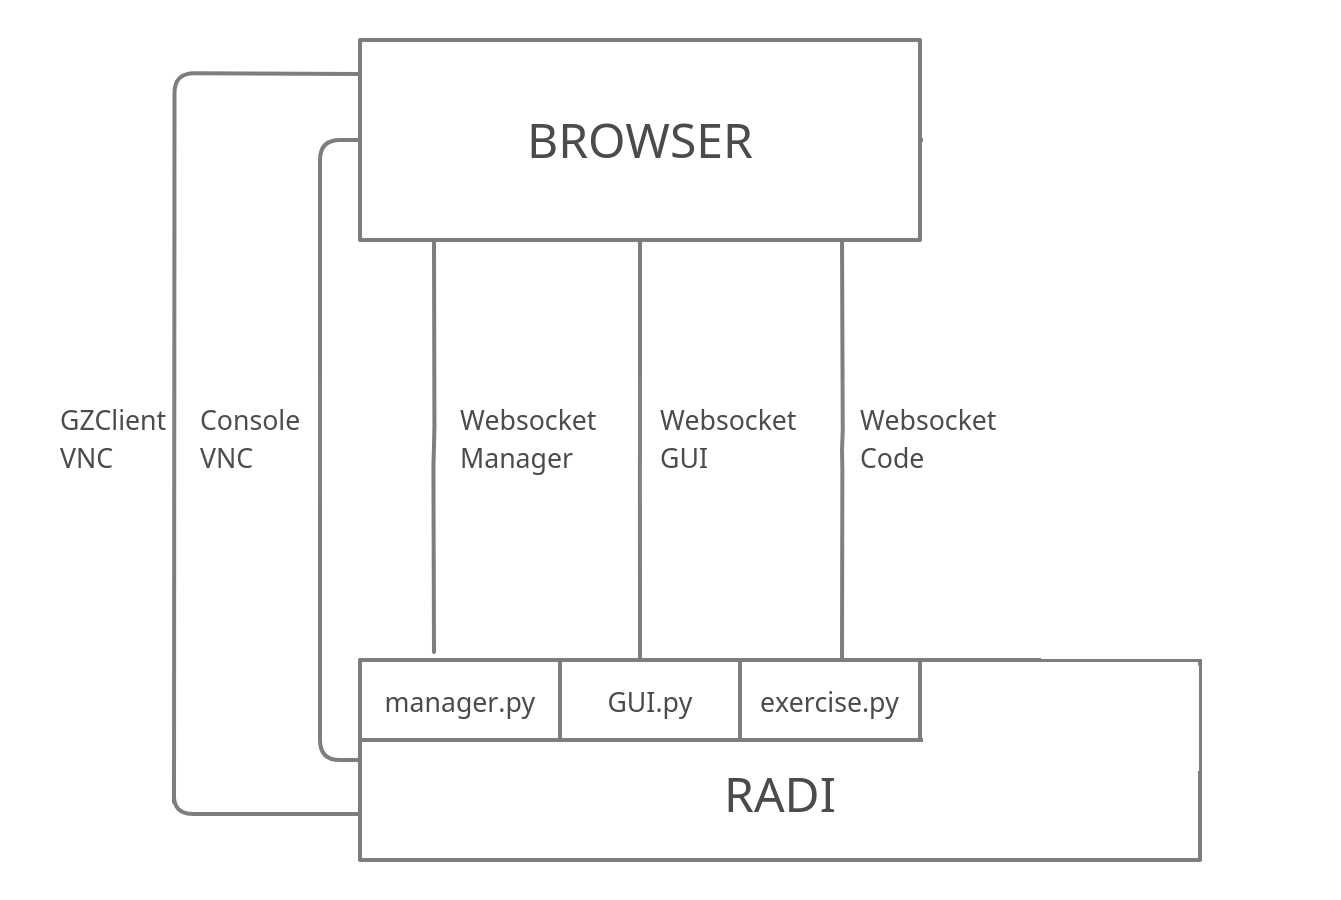
\includegraphics[width=10cm]{img/robotics_academy_architecture.png}
    \caption{Arquitectura de Unibotics.}
    \label{figura:unibotics_architecture}
\end{figure}

\section{Follow Line Game} 
\label{sec:follow_line_game}

\subsection{Diseño}
\label{subsec:follow_line_game_diseño}

Para desarrollar este ejercicio ha sido necesario implementar \emph{software}  en el lado del del cliente especialmente. Se ha diseñado un interfaz de usuario que radica en la simplicidad para el usuario, sin proporcionar un exceso de controles. La plantilla de los ejercicios es común a la mayoría de los ejercicios de la plataforma, pero mediante JavaScript se acondiciona la platilla a los requisitos del ejercicio. Todos los ejercicios tienen en común una barra en la parte superior que contiene una serie de botones para realizar la conexión con el contenedor Docker, que es donde se ejecutará todo lo relativo a la simulación del ejercicio.

\begin{figure}[H]
	\centering
    
\includegraphics[width=15cm]{img/barra_radi.png}
    \caption{Barra conexión con RADI.}
    \label{figura:conexion_radi}
\end{figure}

Volviendo a la parte específica para este ejercicio, tenemos una barra donde se encuentran los controles relativos al control de la simulación, visualización, carga de código e información adicional sobre la simulación.

\begin{figure}[H]
	\centering
    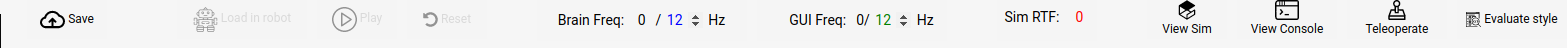
\includegraphics[width=15cm]{img/barra_control.png}
    \caption{Barra de control de la simulación.}
    \label{figura:conexion_radi}
\end{figure}

Bajo las barras de control del ejercicio, se tiene una pantalla que está dividida en dos secciones. La primera sección contiene el selector de circuito, el selector de dificultad y el editor de código. En la segunda sección se encuentra toda la información que se recibe del escenario, esto es, las localizaciones de los coches y sus cámaras, el evaluador automático, el simulador Gazebo y la consola del contenedor.


\begin{figure}[H]
	\centering
    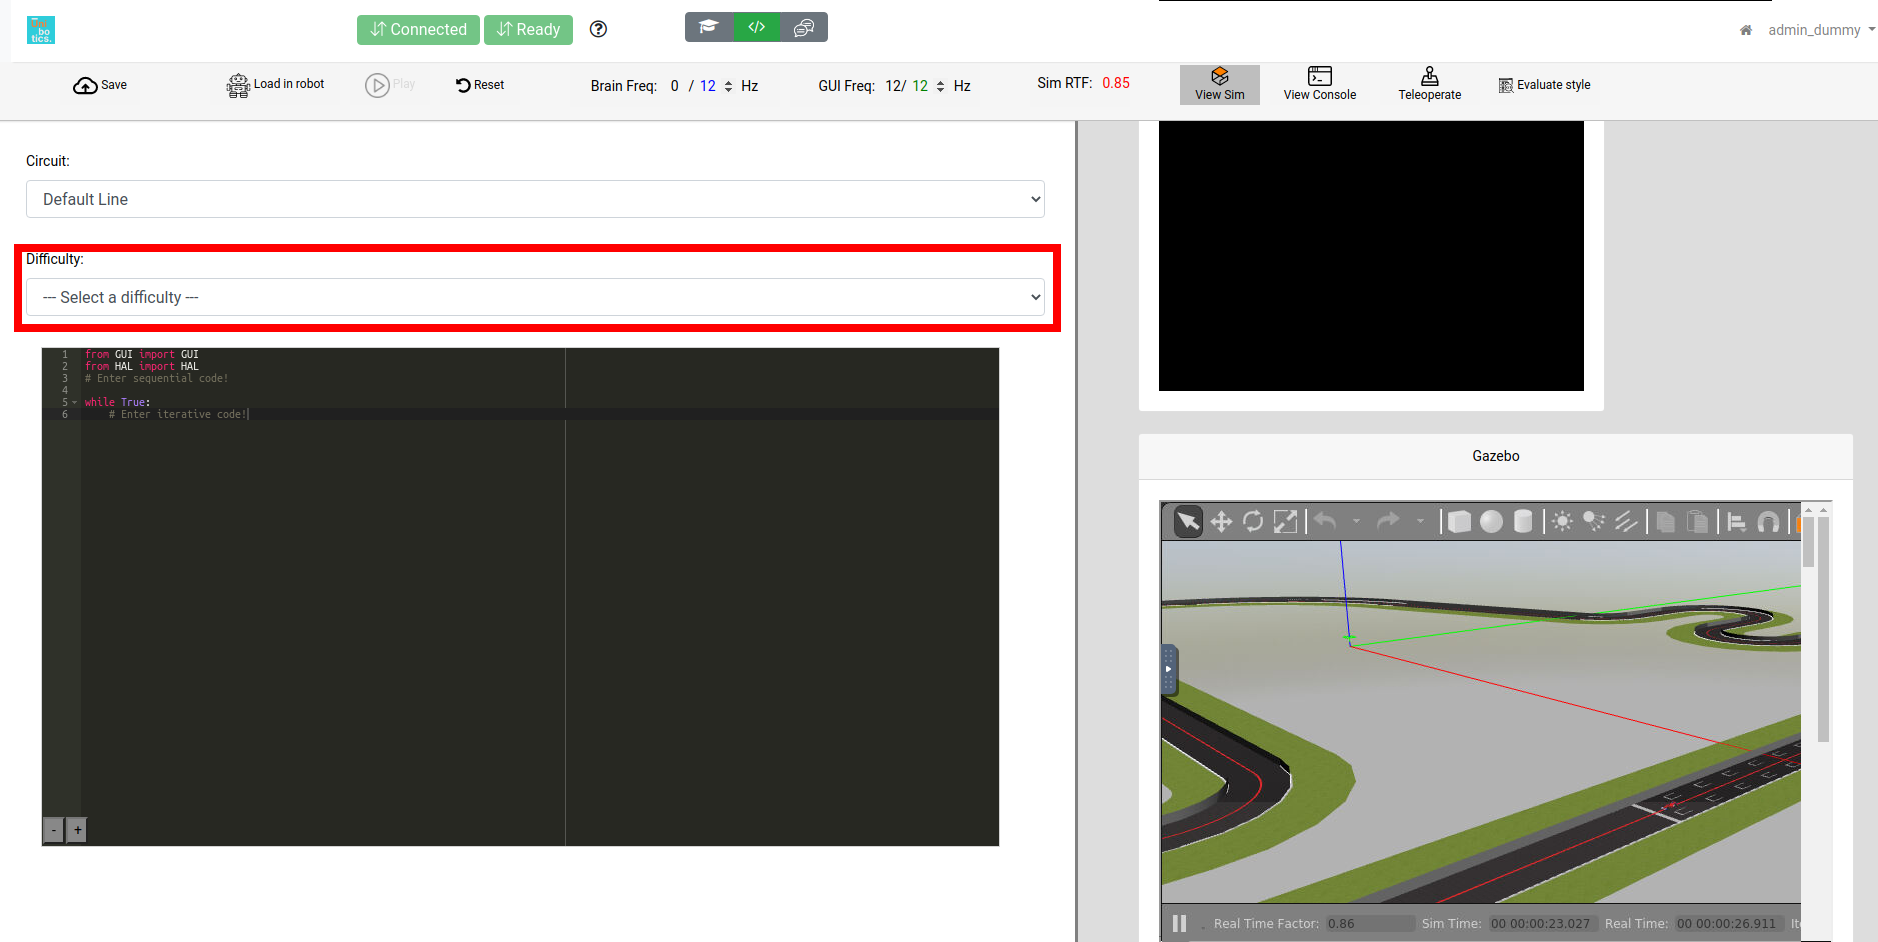
\includegraphics[width=15cm]{img/follow_line_game.png}
    \caption{Plantilla del juego Follow Line.}
    \label{figura:conexion_radi}
\end{figure}

\subsubsection{Robot adversario}
\label{follow_line_game_adversario}


Ha sido necesario añadir un nuevo modelo de robot para que el usuario pueda diferenciar entre su robot y el adversiario. Con lo que se ha modificado el modelo del robot del usuario cambiándolo de color a verde. Esta modificación se ha llevado a cabo mediante \emph{Blender} \footnote{\url{https://www.blender.org/}} y se ha llamado \emph{f1\_guest}.

Una vez creado el nuevo modelo, se ha añadido a los ficheros de declaración de los escenarios de Gazebo, incluyendo el nuevo modelo en una posición del circuito en la que ambos coches se encuentran a la misma distancia. Los ficheros empleados para la configfuración del escenario tienen la siguiente forma:

\begin{lstlisting}
<?xml version="1.0" ?>
<sdf version="1.5">
  <world name="default">
    <gui fullscreen=1></gui>
    <scene>
      <grid>false</grid>
      <sky>
        <clouds>
          <speed>12</speed>
        </clouds>
      </sky>
    </scene>
    <!-- A global light source -->
    <include>
      <uri>model://sun</uri>
      <name>sun_1</name>
      <pose>0 0 1 0 0 0</pose>
    </include>
    <include>
	    <uri>model://simple_circuit</uri>
	    <pose>0 0 0 0 0 0</pose>
    </include>
    <include>
      <uri>model://f1</uri>
      <pose>53.462 -10.734 0.004 0 0 -1.57</pose>
    </include>
    <include>
      <uri>model://f1_guest</uri>
      <pose>-53.2 -6.8 0.004 0 0 -4.85</pose>
    </include>
  </world>
</sdf>
\end{lstlisting}


\subsubsection{Inicio del juego}
\label{subsec:follow_line_game_inicio}

Para llevar a cabo la iniciación del juego es necesario realizar previamente la conexión con el contenedor Docker (\emph{RADI}) donde se va a llevar a cabo toda la ejecución del ejercicio. Una vez realizada esta conexión, se deberá seleccionar el circuito en el que el usuario quiera jugar, seleccionar la dificultad del oponente, y, pulsar el botón \emph{Load in robot}, una vez se hayan cargado los respectivos códigos, se podrá proceder pulsando el botón \emph{Play} para comenzar la ejecución.

Con respecto a las versiones iniciales del reto \emph{Follow Line} de \textbf{Unibotics}, se ha tenido que implementar un cambio dentro del RADI, pues para era necesario poder lanzar el escenario con el circuito seleccionado por el usuario.

Para implementar esta característica, dentro del fichero \emph{manager.py} (encargado del lanzamiento de los ejercicios, comprobar el código mediante PyLint, noVNC, etc), se ha añadido una variable con scope global que contiene un array con todos los ejercicios que requieren el cambio de circuito. De manera que, antes de lanzar un ejercicio se comprueba si es uno de estos, y, si es así, el circuito que se ha obtenido del comando de lanzamiento que llega vía \emph{WebSockets} se emplea para formatear la cadena de texto que contiene la instrucción de lanzamiento del proceso. Esta instrucción de lanzamiento contendrá el nombre del fichero que se corresponde con el modelo del circuito deseado por el usuario, de manera que Gazebo ya sabe qué escenario cargar.

Finalmente, se lanzará este proceso (además de algunos otros como noVNC para mostrar GZClient y la consola), y se avisará al \emph{Front End} que la conexión está lista.

\subsubsection{Selección de circuito}
\label{subsec:follow_line_game_circuito}

El usuario podrá elegir mediante un desplegable uno de los circuitos disponibles para realizar la ejecución del juego, estos circuitos son \emph{Default}, \emph{Montmelo}, \emph{Montreal} y \emph{Nürbugring}. 

\begin{figure}[H]
	\centering
    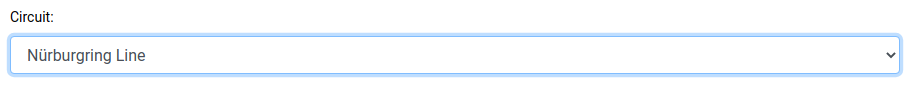
\includegraphics[width=15cm]{img/circuit_selector.png}
    \caption{Selector de circuitos.}
    \label{figura:circuit_selector}
\end{figure}

El circuito \emph{Default} será el escenario por defecto en el que comenzará la simulación, si el usuario selecciona otro, se le comunicará al contenedor Docker, y este se encargará de volver a lanzar la simulación con el escenario seleccionado. Esta comunicación se realiza por medio de WebSockets.

\begin{figure}[H]
	\centering
    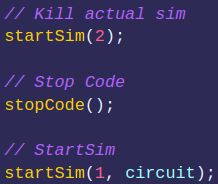
\includegraphics[width=5cm]{img/select_circuit_code.png}
    \caption{Cambio de circuito.}
    \label{figura:circuit_selector}
\end{figure}

Como se puede apreciar en la figura anterior, el código del selector de circuitos se encarga de matar la simulación en curso e iniciar la nueva simulación con el circuito que se obtiene del selector.

\subsubsection{Selección de dificultad}
\label{subsec:follow_line_game_circuito}

El selector de circuitos brinda al usuario un total de tres dificultades diferentes, \emph{Easy}, \emph{Medium} y \emph{Hard}, adicionalmente, el usuario también podrá seleccionar una cuarta dificultad, llamada \emph{Teleoperate} que consiste en que podrá teleoperar el coche del oponente con las teclas de dirección.

\begin{figure}[H]
	\centering
    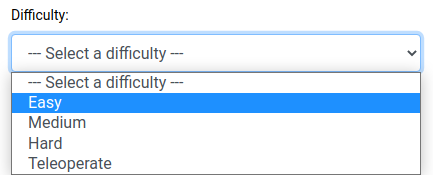
\includegraphics[width=10cm]{img/difficulty_selector.png}
    \caption{Selector de dificultad.}
    \label{figura:difficulty_selector}
\end{figure}

\subsection{Modo teleoperado}
\label{follow_line_game_mode_teleoperado}

En este juego se ha considerado el extra de implementar un modo de teleoperación para ambos vehículos, para brindar al usuario la posibilidad de probar su código ante diversas situaciones y pueda desarrollar un código más robusto, también con el objetivo de que pueda controlar alguno de los dos vehículos en el caso de que se haya quedado atascado. El usuario podrá controlar su vehículo, mediante el botón de teleoperación situado en la barra superior, y el coche oponente seleccionando la dificultar \emph{Teleoperate}, como se ha mencionado antes.

\begin{figure}[H]
  \centering
  \begin{minipage}[b]{0.4\textwidth}
    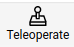
\includegraphics[width=\textwidth,height=\textwidth]{img/teleoperate_off.png}
    \caption{Teleoperación apagada.}
    \label{figura:stun}
  \end{minipage}
  \hfill
  \begin{minipage}[b]{0.4\textwidth}
    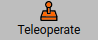
\includegraphics[width=\textwidth,height=\textwidth]{img/teleoperate_on.png}
    \caption{Teleoperación encendida.}
    \label{figura:turn}
  \end{minipage}
\end{figure}

Como se puede apreciar en las figuras, el botón de teleoperación del vehículo del usuario, cambiará de color en función de si la teleoperación está encendida o apagada.

\subsubsection{Implementación del botón de teleoperación}
\label{follow_line_game_mode_teleoperado_impl}

Para llevar a cabo el control de la teleoperación se ha implementado mediante código JavaScript un \emph{listener} para el botón de teleoperación, que se encarga de comprobar si se puede activar el modo, es decir, no se está teleoperando el otro vehículo, cambiar la imagen del botón de teleoperación y añadir el handler correspondiente a los eventos \emph{keyup} y \emph{keydown}.

\begin{figure}[H]
	\centering
    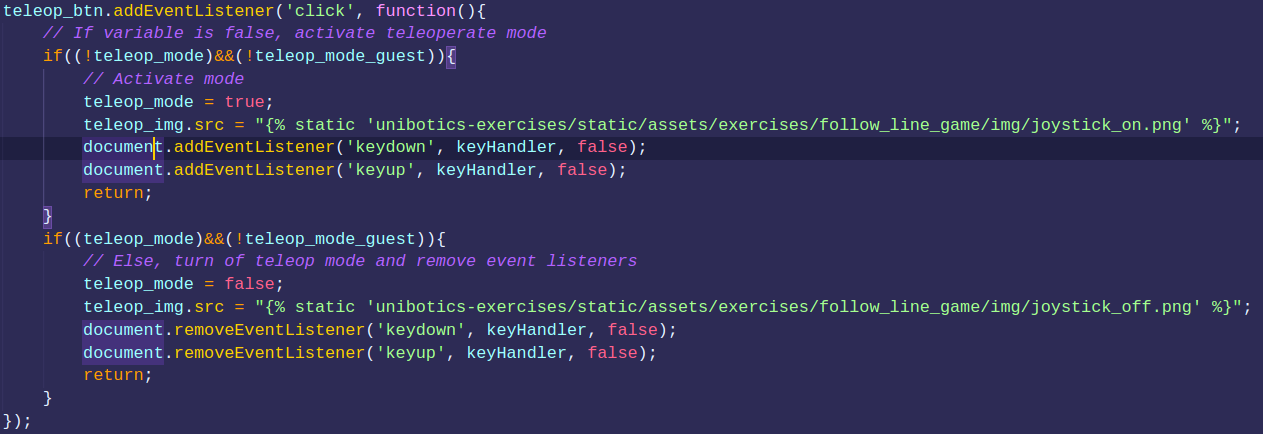
\includegraphics[width=15cm]{img/teleop_mode_code.png}
    \caption{Listener del botón de teleoperación.}
    \label{figura:difficulty_selector}
\end{figure}

El handler que se le asigna a los eventos \emph{keyup} y \emph{keydown} se encarga de determinar cual es la tecla que se ha soltado o pulsado, y, si es una de las flechas de dirección establece un valor constante a la variable de velocidad o giro.

\begin{figure}[H]
	\centering
    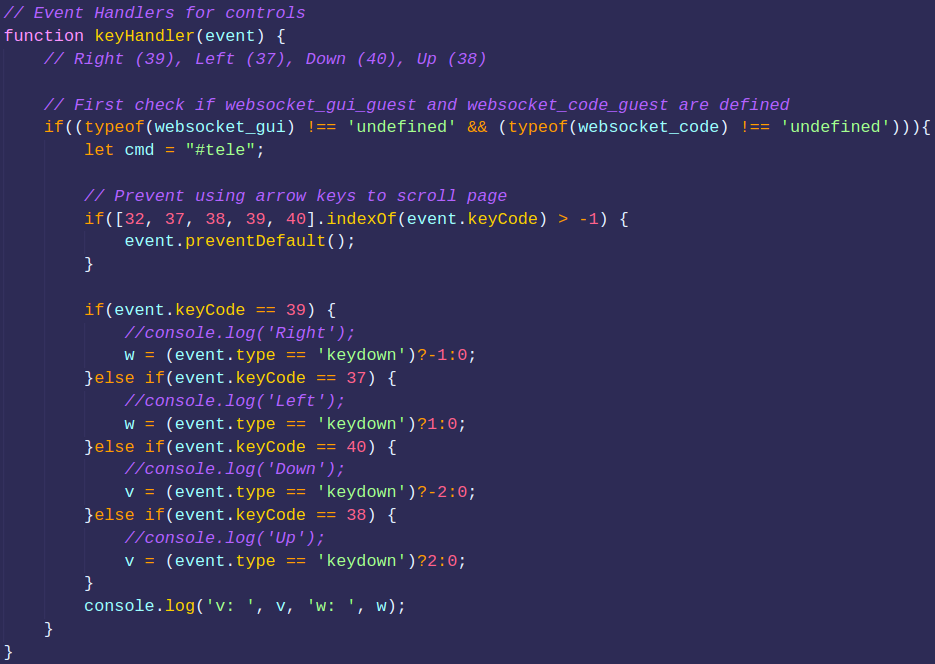
\includegraphics[width=10cm]{img/keyhandler.png}
    \caption{Key Handler.}
    \label{figura:keyhandler}
\end{figure}

Como se puede apreciar en la figura 4.10,los valores de velocidad son asignados a las correspondientes variables de velocidad o de giro. Los valores de estas variables son enviados al contenedor Docker mediante el websocket por el que viaja el código desde el navegador al contenedor.

\subsection{Evaluador automático}
\label{follow_line_game_evaluator}

Este evaluador consiste en mostrar en tiempo real las distancias que hay entre los coches, con el fin de que el usuario pueda competir contra la plataforma. Para cada circuito se han establecido una serie de puntos (\emph{checkpoints}) a lo largo del mismo, que sirven para saber en que lugar se encuentran los robots, y, con esta información poder calcular la distancia que le queda a cada robot para alcanzar al adversario. Estos \emph{checkpoionts} son almacenados en una serie de \emph{arrays}, y, en función del circuito que haya seleccionado el usuario se emplerá el correspondiente.

La información de posición se esta recibiendo con una determinada frecuencia en el tiempo a través del WebSocket \emph{ws\_gui}, este se encarga de actualizar las variables que contienen las posiciones de los robots. A continuación, se ha desarrollado código JavaScript que se encarga de utilizar los valores que contienen estas variables de posición y calcula el checkpoint más cercano a la posición de cada robot y construye los caminos (\emph{paths}) desde un robot hasta el otro. Una vez se obtienen los paths, se calcula la distancia total de estos y se muestra en la interfaz del usuario.

\begin{figure}[H]
	\centering
    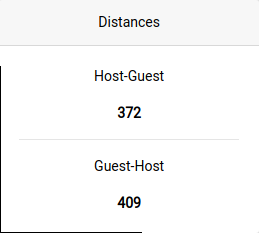
\includegraphics[width=5cm]{img/evaluator_follow_line.png}
    \caption{Evaluador automático.}
    \label{figura:keyhandler}
\end{figure}

\subsection{Carga de código}
\label{follow_line_game_code_load}

Una vez se ha establecido la conexión con \emph{RADI}, se puede proceder a la carga del código. Esta carga se realiza mediante un botón \emph{Load in robot}, que una vez pulsado, se encarga de habilitar el botón \emph{Play} después de haber realizado una comprobación exitosa del código del usuario.

Cuando el usuario procede a realizar la carga del código en los respectivos robots, el código que se ha desarrollado
se obtiene del editor de código situado en la parte izquierda de la pantalla. Para realizar la carga de código de las distintas dificultades, se ha desarrollado un script en \emph{JavaScript} que se encarga de realizar una solicitud al servidor web, pidiendo el código correspondiente con la dificultad seleccionada.

Para que el servidor web pueda proporcionar el código de cada dificultad al navegador web solicitante, se han creado una serie de usuarios con el prefijo de \emph{bot}, que contienen el código correspondiente a cada dificultad. También, ha sido necesaria la creación de un nuevo \emph{endpoint} en el servidor web.

Desde el lado del servidor web, cuando se recibe una solicitud en dicho \emph{endpoint}, este se encarga de determinar cual es la dificultad y el ejercicio del que se está solicitando por medio de los datos aportados en el propio \emph{endpoint}.

Finalmente, unz vez se tienen ambos códigos, estos se envían cada uno por el \emph{WebSocket} que se corresponde con su robot.  

\section{Drone Cat Mouse Game} 
\label{sec:drone_cat_mouse_game}

\subsection{Diseño}
\label{drone_cat_mouse_interface}

Al igual que todos los juegos de la plataforma, estos comparten una plantilla \emph{HTML} con los componentes básicos de un ejercicio, por lo que para el caso de este ejercicio, cabe mencionar que las barras superiores de conexión con \emph{RADI} y de control de la simulacón son similares a las de \textbf{Follow Line Game}.

Bajo el navbar, a mano izquierda se encuentra el editor de código, y a mano derecha, los botones para el control de la ejecución del ratón, el evaluador automático, el simulador \emph{Gazebo} y la consola del contenedor Docker.


\begin{figure}[H]
	\centering
    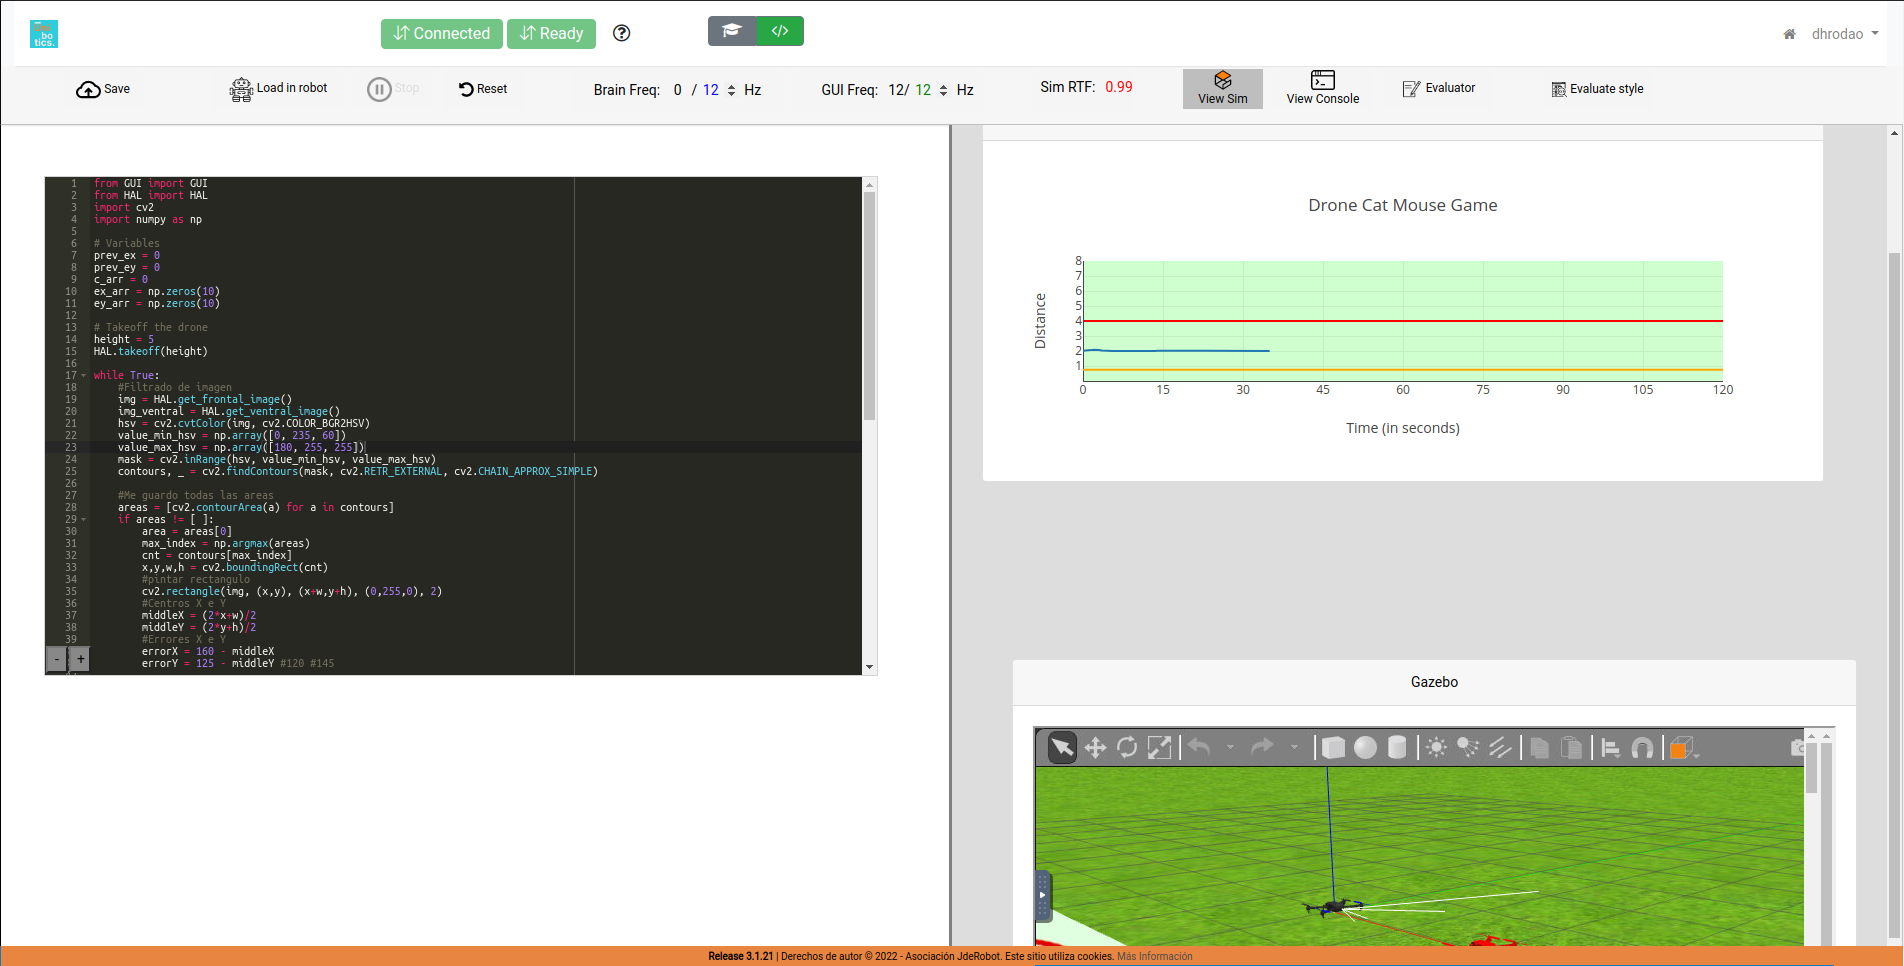
\includegraphics[width=15cm]{img/drone_cat_mouse.png}
    \caption{Plantilla Drone Cat Mouse.}
    \label{figura:keyhandler}
\end{figure}

Por otro lado, la plataforma Unibotics contaba con una versión del reto \emph{Drone Cat Mouse} con una arquitectura en la que, internamente, el \emph{ratón} era instanciado dentro del controlador del robot que se correspondía con el \emph{gato}, y este, se controlaba desde el propio objeto del \emph{gato}.

En la version desarrollada para este trabajo, se han introducido algunos cambios. En primer lugar, se han desacoplado los controladores para los robots, de manera que ahora cada uno es independiente del otro. Esto da lugar a la necesidad de tener dos \emph{WebSockets} para cada robot (inicialmente se tenían únicamente dos \emph{WebSockets} para comunicarse con el \emph{gato}, y este, se encargaba de trasladar la información al \emph{ratón}), \emph{ws\_code} y \emph{ws\_gui} para el \emph{gato} y el \emph{ratón}.

En la versión inicial del ejercicio, el código del ratón, se encontraba almacenado dentro del \emph{RADI}. Actualmente esto se ha cambiado, de manera que el código del \emph{ratón} se pide al \emph{webserver} especificando el ejercicio y la dificultad seleccionada. Este cambio se ha realizado con el fin de seguir el mismo paradigma que con los usuarios, el código de los mismos se recibe desde el \emph{webserver}. Una vez recibido el código, este es enviado al \emph{ratón} por medio del \emph{WebSocket} correspondiente.

\subsubsection{Inicio del juego}
\label{drone_cat_mouse_inicio}

De igual manera que en el juego \emph{Follow Line}, primeramente hay que realizar la conexión con \emph{RADI}, que se encargará de lanzar el proceso del juego, y, una vez se haya establecido la conexión con los \emph{WebSockets}, se avisa al \emph{Front End} de manera que el usuario quede notificado. Posteriormente, puede elegirse la dificultad del ratón, cargar el código del usuario, mostrar \emph{Gazebo} y la consola,  y reanudar la simulación.

\subsubsection{Selección de dificultad}
\label{drone_cat_mouse_difficulty}

El selector de dificultad del \emph{ratón} está situado en la mitad suyperior derecha de la interfaz del usuario junto a los botones de control del mismo. El usuario debe seleccionar primeramente la dificultad deseada mediante el desplegable situado en la mitad derecha de la pantalla. Y, a continuación, pulsar el botón \emph{Load in robot} para proceder a la carga de los códigos.

Para realizar la carga de códigos, primero se obtiene el código del editor de texto situado en la mitad izquierda de la platilla y se envía por el \emph{WebSocket} empleado para comunicarse con el \emph{gato}. A continuación, mediante una peticón HTTP al \emph{WebServer}, se solicita el código del ratón (en función de la dificultad), y finalmente se envía por el \emph{WebSocket} definido para la comunicación  \emph{RADI}-\emph{Ratón}.

\begin{figure}[H]
	\centering
    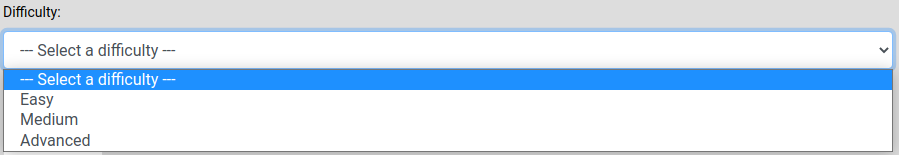
\includegraphics[width=15cm]{img/drone_cat_mouse_difficulty.png}
    \caption{Selector de dificultad Drone Cat Mouse.}
    \label{figura:evaluator_drone}
\end{figure}

\subsection{Evaluador automático}
\label{drone_cat_mouse_evaluator}

En una versión inicial, la plataforma no disponía del \emph{Juego Drone Cat Mouse}, sino, del \emph{Reto Drone Cat Mouse}, es decir, este ejercicio inicialmente no incorporaba un evaluador automático que proporcionase un desafío para el usuario, por lo que se decidió incluir este evaluador para dar lugar al \emph{Juego Drone Cat Mouse}. 

Este evaluador automático consiste en una gráfica que muestra la distancia \emph{Gato}-\emph{Ratón} en el tiempo. La gráfica se genera con una librería de \emph{JavaScript} llamada \emph{Plotly} \footnote{\url{https://plotly.com/javascript/}}, en la cual se muestra la distancia en el eje vertical y el tiempo en el eje horizontal.

\begin{figure}[H]
	\centering
    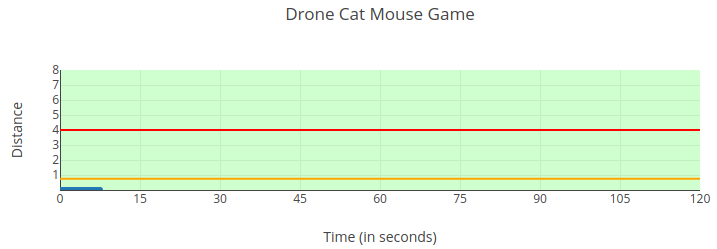
\includegraphics[width=15cm]{img/evaluator_drone_cat_mouse.png}
    \caption{Evaluador Drone Cat Mouse.}
    \label{figura:evaluator_drone}
\end{figure}

\subsection{Carga de código}
\label{drone_cat_mouse_code_load}

Una vez se ha establecido la conexión con \emph{RADI}, se puede proceder a la carga del código. Esta carga se realiza mediante un botón \emph{Load in robot}, que una vez pulsado, se encarga de habilitar el botón \emph{Play} después de haber realizado una comprobación exitosa del código del usuario.

Cuando el usuario procede a realizar la carga del código en los respectivos robots, el código que se ha desarrollado
se obtiene del editor de código situado en la parte izquierda de la pantalla. Para realizar la carga de código de las distintas dificultades, se ha desarrollado un script en \emph{JavaScript} que se encarga de realizar una solicitud al servidor web, pidiendo el código correspondiente con la dificultad seleccionada.

Para que el servidor web pueda proporcionar el código de cada dificultad al navegador web solicitante, se han creado una serie de usuarios con el prefijo de \emph{bot}, que contienen el código correspondiente a cada dificultad. También, ha sido necesaria la creación de un nuevo \emph{endpoint} en el servidor web.

Desde el lado del servidor web, cuando se recibe una solicitud en dicho \emph{endpoint}, este se encarga de determinar cual es la dificultad y el ejercicio del que se está solicitando por medio de los datos aportados en el propio \emph{endpoint}.

Finalmente, unz vez se tienen ambos códigos, estos se envían cada uno por el \emph{WebSocket} que se corresponde con su robot.

%%%%%%%%%%%%%%%%%%%%%%%%%%%%%%%%%%%%%%%%%%%%%%%%%%%%%%%%%%%%%%%%%%%%%%%%%%%%%%%%
%%%%%%%%%%%%%%%%%%%%%%%%%%%%%%%%%%%%%%%%%%%%%%%%%%%%%%%%%%%%%%%%%%%%%%%%%%%%%%%%
% JUEGOS SÍNCRONOS %
%%%%%%%%%%%%%%%%%%%%%%%%%%%%%%%%%%%%%%%%%%%%%%%%%%%%%%%%%%%%%%%%%%%%%%%%%%%%%%%%

\cleardoublepage
\chapter{Juegos Compartidos Síncronos}

En este capítulo se abardarán todos los detalles de los \emph{juegos síncronos}. En una primera parte hablando del diseño e implementación de las plantillas del usuario, para porsteriormente, dirigirnos a los aspectos más técnicos relacionados con las comunicaciones \emph{WebRTC} y el servidor web como servidor de señalización entre los usuarios.

\section{Objetivo}
\label{sync_objective}

En \emph{Unibotics}, se parte de los \emph{ejercicios asíncronos} en lo que únicamente pueden elegirse una serie de dificultades proporcionadas por la plataforma. Con el desarrollo los \emph{ejercicios síncronos} se han querido orientar los juegos hacia un modo más competitivo, de manera que el usuario pueda conectarse con sus amigos y realizar competiciones poniendo en ejecucción sus mejores códigos.

\section{Follow Line Game Síncrono} 
\label{sec:follow_line_game_sync}

\subsection{Diseño}

El juego \emph{Follow Line Síncrono} parte de la plantilla básica que comparten todos los ejercicios. A esta plantilla se le han añadido una serie de extras, como son el chat de texto, la barra de búsqueda de usuarios y los botones de carga de código, del anfitrión y del invitado. Adicionalmente, se ha añadido un botón para ocultar el editor de código con el fin del que el usuario tenga únicamente la vista del chat de texto.

Con respecto la pantalla del usuario invitado, una vez este acepta la invitación proveniente del usuario anfitrión, mediante código \emph{JavaScript}, se ha implementado un sistema que se encarga de ocultar todos los controles y elementos irrelevantes para este extremo de la conexión.
%% AÑADIR CAPTURA DE LA PLANTILLA

Para desarrollar este ejercicio, ha sido necesario implementar \emph{software} tanto en el lado del cliente como en el lado del servidor. Pues los usuarios participantes deben usar el servidor web de \emph{Unibotics} como servidor de señalización para el protocolo \emph{WebRTC}. Una vez ambos extremos se conocen entre sí, se inicia el tráfico \emph{WebRTC}.

Una vez el usuario entra en el ejercicio, automáticamente el navegador se conecta a una ruta del servidor web por medio de \emph{WebSockets} generando una sala de juego. Esta ruta será por medio de la que se van a comunicar los extremos con el servidor de señalización.

Debido a la complejidad de las subredes, ha sido necesaria la incorporación de un servidor \emph{TURN} (Transversal Using Relay NAT) que se encargue de hacer de retransmisor entre los dos extremos una vez se inicia la comunicación \emph{WebRTC}. En la mayoría de casos no es posible realizar una conexión \emph{WebRTC} directa entre los dos extremos (a menos que residan en una red local), esto es debido a que \emph{WebRTC} no es capaz de atravesar un NAT (Network Address Translation).
%% AÑADIR CAPTURA DE ARQUITECTURA

\subsection{Elección de oponente}
\label{sec:follow_line_game_sync_oponente_chat}

Para proporcionar al usuario la elección de un contrincante, se ha implementado una barra de búsqueda de usuarios que permite al anfitrión, escribir el nombre del usuario que desea invitar.

Una vez el usuario realiza la selección del contrincante, la consulta es enviada al servidor web por medio del \emph{WebSocket} de la sala de juego, y, este la reenviará al usuario invitado en caso de que se encuentre en línea y dentro del ejercicio.

En el caso de que el invitado acepte la solicitud, el anfitrión comenzará con la negociación \emph{WebRTC}.

\subsubsection{Barra de búsqueda}

Para poder realizar la conexión entre dos usuarios, el anfitrión debe escribir el login del usuario que quiere invitar en la barra de búsqueda, de manera que se pueda hacer la consulta al servidor web. Se ha desarrollado código \emph{JavaScript} que se encarga de esperar a que se inserte un login y se pulse el botón \emph{"Enter"}, y además, que se encargue de enviar la inserción al servidor web vía el \emph{WebSocket} establecido para la sala del juego.

Una vez el servidor recibe este mensaje por el \emph{WebSocket}, este se encarga de extraer el login del usuario, y mediante el uso de un paquete instalado en el servidor \emph{Django}, llamado \emph{"Django-online-users"}, obtiene los usuarios que hay conectados actualmente, y comprueba si el usuario recibido se encuentra en línea. En el caso en que la búsqueda no sea satisfactoria, se envía un mensaje al usuario anfitrión indicando la imposibilidad de realizar la invitación. Si la búsqueda se realiza con éxito, se envía la invitación a dicho usuario por \emph{WebSocket}.

En el lado del usuario receptor, el navegador recibirá la petición y la mostrará al usuario por medio de un menú de diálogo que le da la posibilidad de aceptar o rechazar la invitación.
%% AÑADIR CAPTURA DE LA INVITACIÓN

Una vez aceptada, se iniciará la conexión \emph{WebRTC}. Y el usuario anfitrión será el encargado de iniciar la simulación y compartir la retransmisión.

\subsubsection{Sección de chat}

Como se ha mencionado antes, la plantilla del juego contiene un chat por el que ambos contrincantes pueden comunicarse. Este chat se ha implementando usando una conexión \emph{WebRTC} y \emph{DataChannels} entre los navegadores, de manera que se reduce la carga de tráfico que atraviesa el servidor web, pues estos mensajes son enviados por medio del canal de datos \emph{peer-to-peer}.

Este sistema se ha desarrollado en la parte del navegador, mediante un \emph{script} en \emph{JavaScript} que contiene toda la configuración para realizar la creación de los \emph{DataChannels}. Además, se ha implementado una función de \emph{callback} (\emph{onDataChannelMessage}) que es ejecutada cuando se recibe un mensaje por el \emph{DataChannel}, esta se encarga de añadir el mensaje al chat.

\subsubsection{Transmisión de datos entre plantillas}

Este \emph{DataChannel} es aprovechado para el paso de más información además de para el envío de los mensajes del chat. De manera que, una vez el anfitrión conecta el \emph{RADI} en su máquina local, por este data channel son enviados todos los datos relativos a la interfaz del usuario, es decir, la vista de pájaro, y el evaluador automático hacia el otro extremo. Adicionalmente, cuando el usuario invitado presione el botón \emph{Play} o el botón de carga de su código, estas órdenes serán enviadas al anfitrión por medio del canal de datos, que será quien las complete.

\subsection{Carga flexible de código}

Para proporcionar la libertad de la carga del código, se ha desarrollado un módulo \emph{software} en \emph{JavaScript} que se encarga de soportar la carga flexible del código.

De esta manera, cada usuario debe cargar su código antes de iniciar la simulación. Con respecto al usuario invitado, se ha desarrollado un sistema que se encarga de avisar al usuario host de que este quiere cargar su código, mediante el \emph{DataChannel} establecido entre ambos. Una vez el host recibe este mensaje, se encarga de pedir el código al \emph{WebServer} y cargarlo en el coche correspondiente. En el lado de la carga de código del host, simplemente, al pulsar el botón de carga de código, se pedirá el código al servidor web y se cargará en el robot correspondiente.

Una vez se carga un código, el botón de carga correspondiente se colorea de verde, de manera que para el usuario es más intuitivo a la hora de comprobar el estado de su código.

Ambos navegadores sincronizan sus interfaces por medio del canal de datos establecido entre los navegadores, enviando mensajes de control que una vez son interpretados, se aplican los cambios a la IU.

\subsection{Ejecución compartida}

Una vez se ha establecido la conexión \emph{WebRTC} entre los usuarios, es necesario realizar la carga de código en los robotos, así como mostrar el estado de carga de los códigos y proporcionar una serie de controles de la ejecución de la sumilación a los usuarios.

\subsubsection{Botones de control de la ejecución}

En ambas interfaces, se encuentran serie de elementos de control de la simulación en común. Estos son:

\begin{itemize}
\item \textbf{Botón \emph{Play}:} ambos usuarios tendrán la posibilidad de iniciar la ejercución del ejercicio una vez se han cargado los códigos en los robots.

\item \textbf{Botón \emph{Reset}:} botón que proporciona a ambos extremos realizar un reseteo del escenario.
\end{itemize}

%% AÑADIR IMAGEN DE LOS BOTONES

Una vez cargados ambos códigos, se habilitará el botón \emph{Play} en ambos extremos. Desde el lado del usuario \emph{invitado}, se ha elaborado un sistema que se encarga de enviar las órdenes al usuario \emph{anfitrión} cuando algún botón es pulsado. Una vez el \emph{emisor} recibe una órden, este se encarga de procesarla y ejecutar las órdenes. De esta manera, ambos usuarios pueden controlar la ejecución de la simulación de manera individual.

\subsubsection{Botones de carga de código}

De manera que los usuarios puedan conocer el estado de carga de sus códigos, se ha implementado un sistema que guarda el estado de carga y realiza una serie de ajustes visuales. Los indicadores de carga son los siguientes:

\begin{itemize}
\item \textbf{Botón de carga de código del anfitrión:} se encuentra únicamente en la plantilla del usuario \emph{emisor}, este elemento es un botón que inicialmente tiene un color rojo, mostrando un estado que representa que no hay ningún código cargado, una vez se carga el código, este botón cambia a un color verde.
\item \textbf{Botón de carga de código del invitado:} se encuentra ambas interfaces, este elemento es un botón que inicialmente tiene un color rojo, mostrando un estado que representa que no hay ningún código cargado, una vez se carga el código, este botón cambia a un color verde en ambos extremos. Este botón no puede ser pulsado en el lado del \emph{emisor}.
\end{itemize}

%% AÑADIR IMAGEN DE LOS BOTONES EN EL HOST Y EL GUEST

El establecimiento de los estados se realiza mediante mensajes vía \emph{WebSockets} entre ambos usuarios. En la plantilla del \emph{anfitrión} es donde se almacenan todas las variables relativas al estado de los códigos, el extremo \emph{invitado} únicamente recibe órdenes vía \emph{WebSockets} para ajustar su interfaz.

\subsubsection{Transmisión vía WebRTC}



%%%%%%%%%%%%%%%%%%%%%%%%%%%%%%%%%%%%%%%%%%%%%%%%%%%%%%%%%%%%%%%%%%%%%%%%%%%%%%%%
%%%%%%%%%%%%%%%%%%%%%%%%%%%%%%%%%%%%%%%%%%%%%%%%%%%%%%%%%%%%%%%%%%%%%%%%%%%%%%%%
% EXPERIMENTOS Y VALIDACIÓN %
%%%%%%%%%%%%%%%%%%%%%%%%%%%%%%%%%%%%%%%%%%%%%%%%%%%%%%%%%%%%%%%%%%%%%%%%%%%%%%%%

\cleardoublepage
\chapter{Experimentos y validación}

Este capítulo se introdujo como requisito en 2019. 
Describe los experimentos y casos de test que tuviste que implementar para validar tus resultados. 
Incluye también los resultados de validación que permiten afirmar que tus resultados son correctos. 


%%%%%%%%%%%%%%%%%%%%%%%%%%%%%%%%%%%%%%%%%%%%%%%%%%%%%%%%%%%%%%%%%%%%%%%%%%%%%%%%
%%%%%%%%%%%%%%%%%%%%%%%%%%%%%%%%%%%%%%%%%%%%%%%%%%%%%%%%%%%%%%%%%%%%%%%%%%%%%%%%
% RESULTADOS %
%%%%%%%%%%%%%%%%%%%%%%%%%%%%%%%%%%%%%%%%%%%%%%%%%%%%%%%%%%%%%%%%%%%%%%%%%%%%%%%%

\cleardoublepage
\chapter{Resultados}

En este capítulo se incluyen los resultados de tu trabajo fin de grado.

Si es una herramienta de análisis lo que has realizado, aquí puedes poner ejemplos de haberla utilizado para que se vea su utilidad.


%%%%%%%%%%%%%%%%%%%%%%%%%%%%%%%%%%%%%%%%%%%%%%%%%%%%%%%%%%%%%%%%%%%%%%%%%%%%%%%%
%%%%%%%%%%%%%%%%%%%%%%%%%%%%%%%%%%%%%%%%%%%%%%%%%%%%%%%%%%%%%%%%%%%%%%%%%%%%%%%%
% CONCLUSIONES %
%%%%%%%%%%%%%%%%%%%%%%%%%%%%%%%%%%%%%%%%%%%%%%%%%%%%%%%%%%%%%%%%%%%%%%%%%%%%%%%%

\cleardoublepage
\chapter{Conclusiones}
\label{chap:conclusiones}


\section{Consecución de objetivos}
\label{sec:consecucion-objetivos}

Esta sección es la sección espejo de las dos primeras del capítulo de objetivos, donde se planteaba el objetivo general y se elaboraban los específicos.

Es aquí donde hay que debatir qué se ha conseguido y qué no. 
Cuando algo no se ha conseguido, se ha de justificar, en términos de qué problemas se han encontrado y qué medidas se han tomado para mitigar esos problemas.

Y si has llegado hasta aquí, siempre es bueno pasarle el corrector ortográfico, que las erratas quedan fatal en la memoria final.
Para eso, en Linux tenemos aspell, que se ejecuta de la siguiente manera desde la línea de \emph{shell}:

\begin{verbatim}
  aspell --lang=es_ES -c memoria.tex
\end{verbatim}

\section{Aplicación de lo aprendido}
\label{sec:aplicacion}

Aquí viene lo que has aprendido durante el Grado/Máster y que has aplicado en el TFG/TFM. Una buena idea es poner las asignaturas más relacionadas y comentar en un párrafo los conocimientos y habilidades puestos en práctica.

\begin{enumerate}
  \item a
  \item b
\end{enumerate}


\section{Lecciones aprendidas}
\label{sec:lecciones_aprendidas}

Aquí viene lo que has aprendido en el Trabajo Fin de Grado/Máster.

\begin{enumerate}
  \item Aquí viene uno.
  \item Aquí viene otro.
\end{enumerate}


\section{Trabajos futuros}
\label{sec:trabajos_futuros}

Ningún proyecto ni software se termina, así que aquí vienen ideas y funcionalidades que estaría bien tener implementadas en el futuro.

Es un apartado que sirve para dar ideas de cara a futuros TFGs/TFMs.


%%%%%%%%%%%%%%%%%%%%%%%%%%%%%%%%%%%%%%%%%%%%%%%%%%%%%%%%%%%%%%%%%%%%%%%%%%%%%%%%
%%%%%%%%%%%%%%%%%%%%%%%%%%%%%%%%%%%%%%%%%%%%%%%%%%%%%%%%%%%%%%%%%%%%%%%%%%%%%%%%
% APÉNDICE(S) %
%%%%%%%%%%%%%%%%%%%%%%%%%%%%%%%%%%%%%%%%%%%%%%%%%%%%%%%%%%%%%%%%%%%%%%%%%%%%%%%%

\cleardoublepage
\appendix
\chapter{Manual de usuario}
\label{app:manual}

Esto es un apéndice.
Si has creado una aplicación, siempre viene bien tener un manual de usuario.
Pues ponlo aquí.

%%%%%%%%%%%%%%%%%%%%%%%%%%%%%%%%%%%%%%%%%%%%%%%%%%%%%%%%%%%%%%%%%%%%%%%%%%%%%%%%
%%%%%%%%%%%%%%%%%%%%%%%%%%%%%%%%%%%%%%%%%%%%%%%%%%%%%%%%%%%%%%%%%%%%%%%%%%%%%%%%
% BIBLIOGRAFIA %
%%%%%%%%%%%%%%%%%%%%%%%%%%%%%%%%%%%%%%%%%%%%%%%%%%%%%%%%%%%%%%%%%%%%%%%%%%%%%%%%

\cleardoublepage

\begin{thebibliography}{X}
	\bibitem{historia} \textsc{Historia de la robótica.}
	\url{https://scielo.isciii.es/pdf/aue/v31n3/v31n3a02.pdf}
	
	\bibitem{javascript} \textsc{Documentación oficial de javascript}
	\url{https://developer.mozilla.org/es/docs/Web/JavaScript}	
	
	\bibitem{django} \textsc{Documentacion oficial de Django}
	\url{https://docs.djangoproject.com}	
	
	\bibitem{webrtc} \textsc{Documentación oficial de WebRTC.}
	\url{https://webrtc.org/}
	
	
	\bibitem{TFM} \textsc{Pablo Moreno. Torneos de programación de robots
en una plataforma online. (2020)}
	\url{https://gsyc.urjc.es/jmplaza/students/tfm-kibotics-torneos-pablo_moreno-2020.pdf}
	
	\bibitem{} \textsc{}
	\url{}
\end{thebibliography}

\end{document}
